\chapter{Deep Generative Learning on Graphs} % Main chapter title
\label{ch:deep-generative-learning-graphs}
In this chapter, we discuss the graph generation problem. The term \quotes{graph generation} is purposedly kept broad, to include a variety of methodologies which learn processes that generate graphs from a set of training examples. This research field originates from generative models of graphs for the theoretical understanding of graph properties, which have been studied thoroughly since the '50s in the field of graph theory. The first known generative model is the  Erd\"{o}s-R\'{e}nyi (ER) model \cite{erdos1959randomgraphs}. The ER model studies random graphs, where the connectivity among graph nodes is modeled independently. This model is useful to study theoretical properties of graphs, such as how the global connectivity of the graph evolves as its size grows. Another historical model of graphs is the  Watts-Strogatz (WS)  model \cite{watts1998smallworld}. The WS model concerns \quotes{small world} graphs, \ie graphs where it is possible to reach any other node in the graph with very short paths, regardless of their ize. This property arises in several real-world graphs such as social and electrical networks. Lastly, the Barab{\'a}si-Albert (BA) model \cite{barabasi1999prefatt}, which models the so-called \quotes{preferential attachment} property, where the connectivity potential of a node is directly proportional to its number of neighbors. While being useful to the study and understanding of graph properties, these models usually fail to generalize to real-world graph distributions, because they can only model one or a limited number of graph properties, and that their parameters cannot be learned from data in general. Other methods such as stochastic block models \citep{airoldi2008mixedstochasticblock}, exponential random graphs \citep{robins2007exponentialrandomgraphs}, and Kronecker graphs \citep{leskovec2010kronecker} can approximate more complex graph distributions such as graphs with communities, but are still limited to specific kinds of graphs and scale poorly to large datasets.
These limitations clearly highlight that, in order to generate graphs for practical applications, a more powerful class of learning models is needed. In this chapter, we review a variety of generative models of graphs based on Deep Learning approaches. The advantages of such models are the possibility to approximate complex distributions efficiently and effectively, and the flexibility to use different generative paradigms to adapt to the task at hand.

\section{The Challenges of Graph Generation}
The problem of generating graph structures from arbitrary distributions is arguably harder than their predictive modeling. Some of the challenges that need to be addressed when designing deep generative models of graphs are related to the complexity of graph spaces. In particular, we report the following:
\begin{itemize}
    \item \emph{size of graphs spaces}. Graphs spaces are combinatorial, and thus very large. For example, the size of the space of undirected graphs with $m$ nodes is ${m \choose 2} = \frac{m(m-1)}{2}$, which becomes very large even for graphs with a moderate number of nodes. Thus, trivial approaches such as exhaustive enumeration are generally intractable. Moreover, real-world graph distributions are usually defined over attributed graphs with variable size, which makes the search space even larger;
    \item \emph{discreteness of graphs spaces}. Graphs are discrete objects. This contrasts with the nature of neural networks, which can backpropagate only through continuous and differentiable objects. Hence, the learning process must be accomodated to work with discrete structures;
    \item \emph{sparsity of graphs spaces}. For most generative tasks, only very small subsets of graph space contain graphs with non-zero probability. Thus, any generative method should be designed to focus on regions where interesting graphs are contained, to avoid efficiency issues;
    \item \emph{complex dependencies}. Most real-world graph have hard structural constraints that are very difficult to enforce on a generative model (which is inherently stochastic). For example, cycle graphs are such that if only one edge is missplaced, the graph is not a cycle anymore;
    \item \emph{non-unique representations}. In general, graphs are invariant under node permutation. Thus, the same graph can be potentially represented by up to $n!$ possible adjacency matrices, depending on the node permutation. This poses constraints on the kind of graph representations a generative model can learn. For example, generative methods that map graphs into a latent space must take into account that different node permutations of the same graph must map to the same latent vector. While invariance to node permutation can be addressed by assuming an order of the graph nodes, this introduces the necessity to maintain order consistency among different graphs.
\end{itemize}

\section{Generative Tasks}
The family of \glspl{dgm} of graphs is flexible enough to model different kinds of generative tasks. Loosely following the taxonomy proposed by \citet{guo2020systematicreviewgenerativegraphs}, we distinguish two main tasks related to graph generation:
\begin{itemize}
    \item \emph{unconditional generation}, where the task is to explicitly learn a distribution $p(\Graph{g})$ over graphs, or some parametrized function that produces samples from it. Here, the term \quotes{unconditional} refers to the fact that the generation starts with drawing a vector $\Vector{z} \in \Real^z$ from some easy to sample prior distribution $p(\Vector{z})$, which is usually assumed to be an isotropic Gaussian or a uniform distribution;
    \item \emph{conditional generation}, where the aim is to learn a conditional distribution $p(\Graph{g} \given \Vector{y})$ with $\Vector{y} \in \Real^y$, or the corresponding parameterized sampling mechanism. The purpose of the conditioning vector is to drive the generative process towards producing a graph with desired characteristics. For example, one might want to generate a graph whose structure resembles that of a graph given as input to the \gls{dgm}. In this case, $\Vector{y}$ is the representation of the conditioning graph.
\end{itemize}
Hereafter, we consider the task of unconditional generation, where we assume access to a dataset of graphs $\Data = \Set{\Graph{g}_i}_{i=1}^n$. Notice from the notation that, at least for the moment, we focus on unattributed graphs. Broadly speaking, defining a \gls{dgm} of graphs requires to specify two components: a \emph{graph decoder}, which takes care of generating a graph, and an end-to-end generative framework used to optimize the model parameters. As regards the latter, common generative frameworks include \glspl{vae}, \glspl{gan}, and flow-based models \citep{rezende2015normalizingflows}. Here, we only describe approaches based on the first two.

\section{Graph Decoders}
The graph decoder is the architectural component that outputs some conditional distribution, which can be sampled to generate a graph. If the framwork in which the decoder is placed allows for inference (such as the \gls{vae}), the conditional is also learned with maximum likelihood; otherwise, (such as with \glspl{gan}) it is used only for sampling, and its parameters are optimized with adversarial training. Ideally, graph decoders should generate permutation invariant graphs; however, this is rarely the case. The major hurdle to devise permutation invariant graph decoders is their computational cost; even though some methods do exist \citep{ermon2020permutationinvariantgraphgeneration}, they are still too inefficient to be deployed in real world scenarios. Thus, in the following, we assume non-invariance.
One particular caveat that needs to be addressed during the training phase of a graph decoder is maintaining the differentiability of the architecture while still generating hard graph samples. This is critical especially in \gls{gan}-like architectures, where the discriminator must be trained with actual graphs. As with sequence generation with \glspl{rnn}, the same techniques (straight-trough gradient estimation, reparameterization, or even reinforcement learning-based techniques \cite{williams1992reinforce}) can be used for this purpose. There are two main paradigms to implement adaptive graph decoders, which we detail in the following.

\subsubsection*{One-shot Decoders}
This class of graph decoders outputs a dense probabilistic adjacency matrix $\ProbAdjMatrix{g} \in \Real^{n \times n}$, where $n$ is the maximum number of nodes allowed. The probabilistic matrix is sampled entry by entry to produce an actual adjacency matrix. The entries of the matrix are modeled as independent Bernoulli variables, which indicate the presence or absence of an edge. In some cases, the elements in the adjacency matrix $a_{ii}$ are modeled as independent Bernoulli variables that specify if a node belongs to the graph or not. In practice, the entries of the matrix are produced by a neural network with sigmoid outputs that predicts an $n \times n$ vector. Thus, the adjacency matrix can be sampled in parallel (hence the term \quotes{one-shot}). Two possible approaches to specify a one-shot decoder are:

\begin{itemize}
    \item \emph{graph-based} decoders, which require a graph representation $\Vector{z}$. In this case, the decoder models the conditional as follows:
    $$p(\ProbAdjMatrix{g} \given \Vector{z}) \approx \prod_{i=1}^n \prod_{j=1}^n p_{\Param}(a_{ij} \given \Vector{z}),$$
    where $p_{\Param}$ is a neural network that predicts the matrix from the graph representation;
    \item \emph{node-based} decoders, which require a matrix of node representations $\Matrix{Z} \in \Real^{n \times z}$. In this case, the decoder models the conditional as follows:
    $$p(\ProbAdjMatrix{g} \given \Matrix{z}) \approx \prod_{i=1}^n \prod_{j=1}^n p_{\Param}(a_{ij} \given \Vector{z}_i, \Vector{z}_j),$$
    where $i$ and $j$ range over the matrix rows. In this case, $p_{\Param}$ is a neural network that takes as input pair of node representations, and applies a sigmoid function to their dot product. The idea is that nodes that are close in representation space should be more likely to be connected.
\end{itemize}
One-shot approaches are usually fast to train and to take samples from. However, they are too simplistic, in that they assume the edges are generated independently (which is usually not the case for real-world graphs). Furthermore, the maximum number of nodes must be pre-specified, which makes them unable to generalize to larger graphs.

\subsubsection*{Autoregressive Decoders}
Autoregressive decoders assume that graphs are generated by some sequential process that involves its set of nodes. Specifically, the generative process is the following:
$$p(\Graph{s}) = \int p(\Graph{s}, \pi)\, d\pi = \int p(\Graph{s} \given \pi)\, q(\pi)\, d\pi,$$
where $\Graph{s}$ are sequences that generate graphs one component at a time, and the order of generation is given directly or indirectly by a nodes permutation drawn from a prior $q(\pi)$. The idea is to decompose the generating sequence autoregressively as follows:
$$p(\Graph{s}) = \int p(\Graph{s}_i \given \Graph{s}_{[<i]}, \pi)\, q(\pi)\, d\pi.$$
However, this requires to integrate over all $n!$ possible node permutations, which becomes intractable for moderately large graphs. An approximate solution to this issue is to assume some ordering and create the sequences before training, as a preprocessing step. Once the sequence are fixed, the chain-rule decomposition becomes tractable:
$$p(\Graph{s}) \approx p_{\Param}^{\pi}(\Graph{s}) = p_{\Param}^{\pi}(\Graph{s}_i \given \Graph{s}_{[<i]}).$$
Depending on the nature of the graph generating sequence, we distinguish four possible approaches to develop autoregressive graph decoders:
\begin{itemize}
    \item \emph{node-based} approaches decompose the graph as a sequence of actions performed on an initially empty graph. These action correspond to decisions such as whether to add a node to the existing graph, and which nodes it must be connected to. In this case, $\Graph{s}_{[<i]}$ is a vector that represents the current state of the graph. For all these models, one has two options as to how to implement the autoregressive network. One approach is to use a hierarchy of \glspl{rnn}: one keeps track of the state of the nodes added to the graph, and the other is responsible to connect newly added nodes to the current graph, given the state of the first \citep{you2018graphrnn}. The other choice is to update the state of the current graph with a \gls{dgn}, which is passed to the networks responsible of deciding which action to perform \citep{li2018learningdeepgmg};
    \item \emph{edge-based} approaches decompose the graph as a sequence of edges. To produce an ordered sequence of edges, one must first order its nodes, then label the nodes with progressive integers, and then sort its set of edges in lexicographic order. In this case, $\Graph{s}_{[<i]}$ represents the state of the graph indirectly, by keeping memory of the edges of the sequence already generated. These approaches are mostly implemented with \glspl{rnn} \citep{goyal2020graphgen,bacciu2019edgegraphgenrnn};
    \item \emph{rule-based} approaches can be applied in cases where the graph generation can be decomposed in a sequence of production rules over some known grammar (\eg molecules or computer programs) \citep{kusner2017grammarvae,dai2018sdvae}. In this case, the model generates a sequence of production rules to construct a desired graph;
    \item \emph{motif-based} approaches decompose the graph as a sequence (or even a tree) of \emph{motifs}, \ie very small and manageable subgraphs, which are combined together adaptively. Here, the challenge is mainly how to decompose the graphs into sequences of motifs,
\end{itemize}
A special kind of sequential decomposition for graphs is the \gls{smiles} linearization applied to molecules. We shall define the SMILES more precisely in Section \ref{subsec:smiles}; for the moment, it is sufficient to say that the SMILES encoding of a molecule is a string of ASCII characters that represents its structure. When a domain-specific linearization techniques such as SMILES are not available, the sequences representing the graph generative process are constructed based on some node ordering strategy. One general strategy to do so is to choose one node at random, then visit the graph nodes with a depth-first or breadth-first traversal. The order by which the nodes are visited is used to determine the order of the elements in the sequences. Clearly, this approach is not optimal since it heavily depends on the starting node, and may produce very different sequences for different starting node choices. However, it has been shown to work empirically \citep{you2018graphrnn,li2018learningdeepgmg,bacciu2019edgegraphgenrnn,goyal2020graphgen}. The pros and cons of autoregressive decoders are orthogonal to those of one-shot decoders: briefly, they allow to generate variable-sized graphs seamlessly, and they can model dependencies between nodes and edges by means of the autoregressive property. However, both training and sampling processes are slower in terms of computational time, because the graphs are reconstructed one sequence element at a time and not in parallel.

\section{Performance Evaluation}\label{sec:evaluation-generative-graphs}
The desired end result of training a generative model is that the structure of samples generated by the network should resemble that of graphs in the training set, without being identical. This is a very different setting with respect to predictive tasks, since the samples of a generative model do not exist until they are generated. Hence, one does not have access to held-out ground truth values to measure generalization. Furthermore, the model can very easily obtain deceptive-looking performances by learning to replicate training graphs exactly, or repeating the same graph typology over and over. Thus, one critical aspect of using generative models of graphs is how to assess performances. Below, we define two broad classes of metrics that allow the evaluation of graph models, assuming the availability of a training sample $\TrainingSample \subseteq \Data = \Set{\Graph{g}}_{i=1}^n$ , and a collection\footnote{Here, we use the term \quotes{collection} to indicate a multiset, meaning that it can possibly contain duplicate elements.} $\GeneratedSample = \Set{\Graph{g'}}_{i=1}^m$ of samples generated by the model.

\subsection{Quantitative Metrics}
\emph{Quantitative} metrics measure the rate at which the generative model produces diverse and heterogeneous graphs, without taking into account structural similarity. The three main quantitative matrics considered in the literature are:
\begin{itemize}
    \item \emph{novelty} measures the ratio of generated samples that are not training samples. A high novelty indicates that the model has not learned to replicate training graphs. Formally, it is measured as $1 - \frac{|\GeneratedSample \Inter \TrainingSample|}{|\TrainingSample|}$;
    \item \emph{uniqueness} measures the ratio of unique graphs with respect to the total number of graphs generated. A low uniqueness rate might indicate that the model has overfit one specific typology of graph. To calculate uniqueness, one first checks every graph for isomorphism with every other graph in the generated sample, removing them. If the resulting set of unique graphs is indicated by $\UniqueSample$, uniqueness can be simply calculated as $\frac{|\UniqueSample|}{|\GeneratedSample|}$.
    \item \emph{validity} measures the ratio of generated graphs that respect some validity constraint, out of the total number of graphs generated. To calculate validity, one needs to check wheter every generated graph satisfies some structural constraint or not (\eg the presence of a cycle). If $\ValidSample$ is the collection of graphs that satisfy the structural constraints, validity is calculated as $\frac{|\ValidSample|}{|\GeneratedSample|}$. This metric is particularly useful in molecular generation tasks, since chemically invalid molecules are useless. When assessing validity is required, novelty and uniqueness are usually conditioned on validity first, meaning that the all the invalid graphs are removed from $\GeneratedSample$ before calculating these two metrics.
\end{itemize}

\subsection{Qualitative Metrics}
Quantitative metrics give only one side of the spectrum relatively to how a generative model is performing. For example, assessing novelty alone might be misleading, since a high novelty rate can also be associated to underfitting (meaning that the model generates graphs very different from the training sample, which are trivially novel). Thus, a proper evaluation of generative models must also include a series of metrics that consider the structural properties of the generated graphs. We call such metrics \emph{qualitative}. The framework under which qualitative metrics are assessed consists of comparing the empirical distribution of a certain graph property in the training sample, to the empirical distribution on the generated sample. Given a generic graph with $d$ nodes, coming from one of the two samples indifferently, a relevant subset of such properties includes:
\begin{itemize}
    \item node degree distribution, that is, an $d$-dimensional vector where each position contains the degree of the corresponding node. Notice the the length of the vector may differ across different graphs, since their number of nodes may change;
    \item clustering coefficient distribution. The clustering coefficient of a node $v$ is defined as the ratio between the number of actual connections between neighbors of $v$ out of the total number of possible connections. In other words, it is a relative measure of how many \quotes{closed triangles} (fully connected graphs with three nodes) the node is part of. Similarly to the node degree distribution, it consists of an $d$-dimensional vector where each position contains the clustering coefficient of the corresponding node;
    \item number of nodes of the graph, which is a single integer;
    \item number of edges of the graph, which is again a single integer;
    \item average orbit counts. Orbits are subgraph with 4 nodes. Counting orbits in a graph can be viewed as a generalization of the clustering coefficient to 4-node subgraphs instead of triangles. In practice, it consists in a $dk$-dimensional vector, where $k$ is the number of orbits considered;
    \item \gls{nspdk} \citep{costa2010nspdk}, which measures the similarity between two graphs by counting the number of matching induced subgraphs between them. The subgraphs are derived node-wise, by considering neighborhoods of a node comprising nodes at increasing path lengths. Differently from the other qualitative metrics, the \gls{nspdk} provides a global measure of similarity between graphs, since it is based on multiple subgraph matchings. In practice, it is a vector of length $m-1$ ($n-1$, respectively), where each position measures the similarity of the graph with another graph in the sample.
\end{itemize}
Once the graph properties are calculated for each graph in the sample, there are two options to measure the distance between the empirical distribution of the training sample versus the generated sample, based on their respective number of elements:
\begin{itemize}
    \item if $n = m$, one can compute their empirical \gls{kld} as follows:
    $$\EKLD{\Prop(\GeneratedSample)}{\Prop(\TrainingSample)} = \frac{1}{n} \sum_{i=1}^{n} \Prop(\Graph{g}_{(i)}) \log \Par{\frac{\Prop(\Graph{g'}_{(i)})}{\Prop(\Graph{g}_{(i)})}},$$
    where $\Prop$ is one of the properties mentioned above;
    \item if $n \neq m$, one can either concatenate all the values of the property for each each in the sample, and then fit a histogram with an equal number of bins to make their length match in order to apply the empirical \gls{kld}. Another, more general, approach to compare distribution when the two samples have different lengths is to compute their \gls{mmd} \citep{gretton2012mmdkernel}. Intuitively, the \gls{mmd} measures the distance between two distributions as the sum of the distances of between their matching moments. The computation of these distances can be generalized to an infinite space of moments by applying a kernel trick \citep{smola2008kernels}.
\end{itemize}

\section{A Model for Edge-Based Graph Generation}
\subsection{Introduction}
In this section, we present an original contribution. Specifically, we introduce a novel generative model for graphs, capable of generating unattributed graphs coming from very different graph distributions. We transform graphs into sequences of ordered edges, from which we extract two sequences derived from the edge endpoints. We use a model composed of two \glspl{rnn} to learn the probability distribution of such sequences: the first is an autoregressive network which generates a specification of the graph to produce, which is completed into a graph by the second network. We experiment extensively with the proposed model, comparing its performances with a pool of baselines, one of which is a \gls{dgm} of graphs that holds state-of-the-art performances at the generative task. The experimental framework has been designed to evaluate the proposed model on concerning both quantitative and qualitative aspects, as discussed in Section \ref{sec:evaluation-generative-graphs}. Our experiments demonstrate that, under our evaluation framework, the proposed model is able to perform at, and sometimes surpass, the state-of-the-art in the task of generating graphs coming from very different distributions. Furthermore, we study the effect of changing the order of the edge sequence by experimenting with different node orderings. We show that the chosen node ordering strategy  is more effective for learning complex dependencies than the alternatives, and produces graphs of better quality.

\subsection{Methods}
In this section, we present the methodologies used to develop the model. In particular, we formally introduce the concept of ordered edge sequences, we develop the model,and  we show how it is trained and how graph generation is achieved.

\subsubsection*{Ordered Edge Sequences}
Let $\Graph{g} = \Tuple{\Nodes{g}, \Edges{g}}$ be a fully connected unattributed graph with $n$ nodes and $m$ edges. We assume $\Graph{g}$ is undirected for simplicity, without loss of generality. Let $\gamma: \Nodes{g} \shortrightarrow \Natural_{+}$ be a bijective node labelling function which assigns a unique positive integer (which we call node ID) to each node in the graph; thus, $\gamma$ defines a total order over the nodes of $\Graph{g}$. The \emph{ordered edge sequence} $\Cal{S}$ of graph $\Graph{g}$ is the sequence of pairs:
$$\OES{S}_{\Graph{g}} = ((s_1, e_1), (s_2, e_2), \ldots, (s_m, e_m)),$$
where $(\gamma^{-1}(s_i), \gamma^{-1}(e_i)) \in \Edges{g}$, and such that it is ordered lexicographically according to the IDs assigned to the nodes, \ie $(s_i,e_i) \leq (s_j,e_j)$ if and only if $s_i < s_j$, or $s_i = s_j$ and $e_i \leq e_j$. Given a generic pair $(s_i,e_i) \in \OES{S}_{\Graph{g}}$, we call $s_i \in \Natural_{+}$ its \emph{starting node} and $e_i \in \Natural_{+}$ its \emph{ending node}. Finally, let us define the \emph{starting sequence} $\Start{\OES{S}_{\Graph{g}}} = (s_1, s_2, \ldots, s_m)$, the sequence corresponding of starting nodes ordered as in $\Graph{e}$, and analogously, the \emph{ending sequence} $\End{\OES{S}_{\Graph{g}}} = (e_1, e_2, \ldots, e_m)$, corresponding to the ending nodes ordered as in $\OES{S}$. For conciseness, let us omit the dependece of $\OES{S}_{\Graph{g}}$ on the graph $\Graph{g}$, and of the starting and ending sequences from $\OES{S}_{\Graph{g}}$ whenever they are clear from the context. Clearly, the choice of the labelling function $\gamma$ is critical in determining the ordered sequence of a graph. Given the graph $\Graph{g}$, we choose to implement $\gamma$ with the following algorithm:
\begin{itemize}
    \item first, select a node $v_1$ at random from its set of nodes $\Nodes{g}$, and set its node ID as $\gamma(v_1) = \SF{1}$;
    \item then, traverse the graph in breadth-first order. Let $V = (v_2, v_3, \ldots, v_{n})$ be the ordered sequence of nodes visited during the traversal, excluding $v_s$. Assign node ID $\gamma(v_i) = \SF{i},\, \forall v_i \in V,\, i=2, \ldots, n$.
\end{itemize}
Assuming graph $\Graph{g}$ has the structure shown in Figure \ref{fig:example-graph}, and that node $v_1$ is chosen as the root node for the visit, an example of how the graph nodes are labeled by $\gamma$ is shown in Figure \ref{fig:labeled-graph}. Notice that $\gamma$ is trivially bijective, since it assigns a different integer to each node. Once the nodes are labeled, the ordered edge sequence of $\Graph{g}$ is $\OES{S} = (\OElem{1}{2},\OElem{1}{3},\OElem{1}{4},\OElem{3}{4},\OElem{3}{5})$, with $\tau_S = (\SF{1},\SF{1},\SF{1},\SF{3},\SF{3})$ and $\tau_E = (\SF{2},\SF{3},\SF{4},\SF{4},\SF{5})$. Notice that the graph can be readily reconstructed from its orderd edge sequence by first applying the inverse function $\gamma^{-1}$ to each element of its pairs to obtain $\Edges{g}$, which in turn gives $\Nodes{g}$ since we assumed that $\Graph{g}$ is fully connected.

\begin{figure*}[h!]
    \begin{subfigure}[b]{0.48\linewidth}
        \centering
        \resizebox{.8\textwidth}{!}{

\tikzset{every picture/.style={line width=0.75pt}} %set default line width to 0.75pt

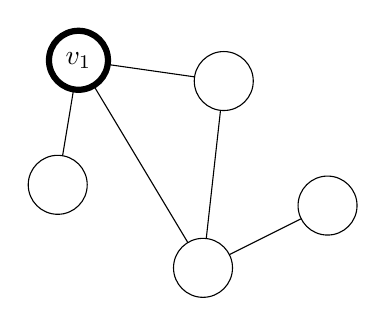
\begin{tikzpicture}[x=0.75pt,y=0.75pt,yscale=-1,xscale=1]
%uncomment if require: \path (0,169); %set diagram left start at 0, and has height of 169


% Text Node
\draw  [line width=2.25]   (45, 32) circle [x radius= 14.21, y radius= 14.21]   ;
\draw (45,32) node   [align=left] {\begin{minipage}[lt]{13.600000000000001pt}\setlength\topsep{0pt}
\begin{center}
$\displaystyle v_{1}$
\end{center}

\end{minipage}};
% Text Node
\draw    (115, 42) circle [x radius= 14.21, y radius= 14.21]   ;
\draw (115,42) node   [align=left] {\begin{minipage}[lt]{13.600000000000001pt}\setlength\topsep{0pt}
\begin{center}
$ $
\end{center}

\end{minipage}};
% Text Node
\draw    (35, 92) circle [x radius= 14.21, y radius= 14.21]   ;
\draw (35,92) node   [align=left] {\begin{minipage}[lt]{13.600000000000001pt}\setlength\topsep{0pt}
\begin{center}
$ $
\end{center}

\end{minipage}};
% Text Node
\draw    (105, 132) circle [x radius= 14.21, y radius= 14.21]   ;
\draw (105,132) node   [align=left] {\begin{minipage}[lt]{13.600000000000001pt}\setlength\topsep{0pt}
\begin{center}
\end{center}

\end{minipage}};
% Text Node
\draw    (165, 102) circle [x radius= 14.21, y radius= 14.21]   ;
\draw (165,102) node   [align=left] {\begin{minipage}[lt]{13.600000000000001pt}\setlength\topsep{0pt}
\begin{center}
$ $
\end{center}

\end{minipage}};
% Connection
\draw    (42.66,46.02) -- (37.34,77.98) ;
% Connection
\draw    (59.07,34.01) -- (100.93,39.99) ;
% Connection
\draw    (52.31,44.19) -- (97.69,119.81) ;
% Connection
\draw    (113.43,56.13) -- (106.57,117.87) ;
% Connection
\draw    (117.71,125.64) -- (152.29,108.36) ;

\end{tikzpicture}}
        \caption{}
        \label{fig:example-graph}
    \end{subfigure}
    \begin{subfigure}[b]{0.48\linewidth}
        \centering
        \resizebox{.8\textwidth}{!}{

\tikzset{every picture/.style={line width=0.75pt}} %set default line width to 0.75pt

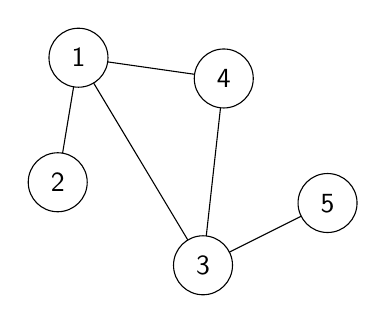
\begin{tikzpicture}[x=0.75pt,y=0.75pt,yscale=-1,xscale=1]
%uncomment if require: \path (0,181); %set diagram left start at 0, and has height of 181


% Text Node
\draw    (45, 42) circle [x radius= 14.21, y radius= 14.21]   ;
\draw (45,42) node   [align=left] {\begin{minipage}[lt]{13.600000000000001pt}\setlength\topsep{0pt}
\begin{center}
$\displaystyle \mathsf{1}$
\end{center}

\end{minipage}};
% Text Node
\draw    (115, 52) circle [x radius= 14.21, y radius= 14.21]   ;
\draw (115,52) node   [align=left] {\begin{minipage}[lt]{13.600000000000001pt}\setlength\topsep{0pt}
\begin{center}
$\displaystyle \mathsf{4}$
\end{center}

\end{minipage}};
% Text Node
\draw    (35, 102) circle [x radius= 14.21, y radius= 14.21]   ;
\draw (35,102) node   [align=left] {\begin{minipage}[lt]{13.600000000000001pt}\setlength\topsep{0pt}
\begin{center}
$\displaystyle \mathsf{2}$
\end{center}

\end{minipage}};
% Text Node
\draw    (105, 142) circle [x radius= 14.21, y radius= 14.21]   ;
\draw (105,142) node   [align=left] {\begin{minipage}[lt]{13.600000000000001pt}\setlength\topsep{0pt}
\begin{center}
$\displaystyle \mathsf{3}$
\end{center}

\end{minipage}};
% Text Node
\draw    (165, 112) circle [x radius= 14.21, y radius= 14.21]   ;
\draw (165,112) node   [align=left] {\begin{minipage}[lt]{13.600000000000001pt}\setlength\topsep{0pt}
\begin{center}
$\displaystyle \mathsf{5}$
\end{center}

\end{minipage}};
% Connection
\draw    (42.66,56.02) -- (37.34,87.98) ;
% Connection
\draw    (59.07,44.01) -- (100.93,49.99) ;
% Connection
\draw    (52.31,54.19) -- (97.69,129.81) ;
% Connection
\draw    (113.43,66.13) -- (106.57,127.87) ;
% Connection
\draw    (117.71,135.64) -- (152.29,118.36) ;

\end{tikzpicture}}
        \caption{}
        \label{fig:labeled-graph}
    \end{subfigure}
    \caption{({\scriptsize A}): an example graph, where the starting node $v_1$ of the labelling algorithm is marked with a thicker border. ({\scriptsize B}): the same graph, where nodes are labeled according to a breadth-first visit of the graph rooted at $v_1$.}
    \label{fig:labelling-example}
\end{figure*}

\subsubsection*{Model}
Our goal is to model $p(\OES{S})$, the probability of ordered edge sequences, using a dataset $\Data = \Set{\OES{S}_{(i)}}_{i=1}^n$. Our key observation is that any ordered edge sequence $\OES{S}$ is uniquely defined by its starting and ending sequences. Therefore, instead of working on the ordered edge sequence directly, we work on their starting and ending sequences. Specifically, we model the probability of sampling $\OES{S}$ from $p(\OES{S})$ as follows:
$$p(\OES{S}) = p(\tau_S, \tau_E) = p(\tau_E \given \tau_S)\, q(\tau_S) = \prod_{i=1}^{|\OES{S}|} p(e_i \given s_i)\, \prod_{j=1}^{|\OES{S}|} q(s_j \given s_{[<j]}).$$
Intuitively, the generative process specified by the distribution is the following:
\begin{itemize}
    \item first, one samples $\tau_S$ from a prior probability $q(\tau_S)$, which is modeled autoregressively;
    \item once $\tau_S$ is available, it is used to condition the prediction of the ending sequence $\tau_E$.
\end{itemize}
Once both $\tau_S$ and $\tau_E$ are available, the ordered edge sequence (and thus, the corresponding graph) an be reconstructed simply pairing their elements. Here, we make an important remark. Notice that the the probability of $q(\tau_S)$ is modeled autoregressively, while the conditional $p(\tau_E \given \tau_S)$ is not. This means that to generate a sequence, the only stochastic part in the model relates to $q(\tau_S)$, while predicting $\tau_E$ is deterministic once $\tau_S$ is known. One possible interpretation of $q(\tau_S)$ is that it acts as a \quotes{soft prior} of the structure of the graph: in fact, it specifies a subset of relevant nodes for the generation and their degree, expressed as the number of times they appear in the starting sequence. The conditional $p(\tau_E \given \tau_S)$ uses this information to \quotes{complete} the graph based on the information provided by the prior.

\subsubsection*{Training}
The model specified above is implemented as two \glspl{rnn} in cascade, which we refer to as $q_{\EncParam}$ and $p_{\DecParam}$ respectively. The two sequences (starting and ending) are first encoded as sequences of $(k+2)$-dimensional one-hot vectors, where $k$ is the largest node ID assigned by $\gamma$ to any node in the dataset, and $+2$ is added for the start of sequence and end of sequence tokens. We indicate the one-hot encoded starting sequence with the notation $\Vector{s} = (\Elem{s}{1}, \ldots, \Elem{s}{|\tau_S|}, \EOS)$, where $\Elem{s}{i} \in \Real^{k+2}$, and analogously, we use $\Vector{e} = (\Elem{e}{1}, \ldots, \Elem{e}{|\tau_E|})$ for the one-hot encoded ending sequence, with $\Vector{e}_i \in \Real^{k+2}$. Notice that an end of sequence token is added to $\Vector{s}$: when it is predicted, the autoregressive process that yields $\Vector{s}$ is interrupted. Our dataset is has thus the following form: $\Data = \Set{(\Vector{s}_{(i)}, \Vector{e}_{(i)})}_{i=1}^n$. Focusing on a single training pair $(\Vector{s}, \Vector{e})$, we explain the feed-forward phase of the network. Firstly, the sequence $\Vector{s}$ is processed by $q_{\EncParam}$. Given an element $\Elem{s}{i} \in \Vector{s}$, the per-element output of $q_{\EncParam}$ is obtained as follows:
\begin{align*}
    \Elem{h}{i} &= \Op{GRU}_{\EncParam}(\Elem{h}{i-1}, \Matrix{E}^{\Transpose}\Elem{s}{i-1})\\
    \Elem{o}{i} &= \softmax(\Matrix{V}_{\EncParam}\Elem{h}{i} + \Vector{b}_{\EncParam}).
\end{align*}
In the formula above, $\Matrix{E} \in \Real^{k \times h}$ is an \emph{embedding matrix} whose entries are learnable, and the dot product selects the column of $\Vector{E}$ corresponding to the embedding of the node ID assigned to $\Elem{s}{i}$. Furthermore, $\Elem{h}{i} \in \Real^h$ is a hidden state, $\Op{GRU}_{\EncParam}$ is a multi-layer GRU network, $\Matrix{V}_{\EncParam} \in \Real^{h \times (k+2)}$ and $\Vector{b}_{\EncParam} \in \Real^{k+2}$ are the weights of the softmax output layer, and $\Elem{o}{i}$ is an output distribution over all the possible node IDs. The process is initialized by setting $\Elem{s}{0} = \SOS$ and $\Elem{h}{0} = \Zeros$. We use teacher forcing, meaning that, at each step, the input of the network is the ground truth value taken from $\Vector{s}$, rather than the output predicted by the network. Lastly, the output $\Elem{o}{i}$ is compared to the ground truth value $\Elem{s}{i}$ using the \gls{ce} loss function. For the whole starting sequence, the computed loss is the following:
$$\Loss(\EncParam, \Vector{s}) = \frac{1}{|\Vector{s}|+1} \sum_{i=1}^{|\Vector{s}|+1} q_{\EncParam}(\Elem{s}{i} \given \Elem{s}{<i}) = \frac{1}{|\Vector{s}|+1} \sum_{i=1}^{|\Vector{s}|+1} \mathrm{CE}(\Elem{s}{i}, \Elem{o}{i}).$$
After the starting sequence $\Vector{s}$ has been processed by $q_{\EncParam}$, the control flow passes onto $p_{\DecParam}$. The function computed by $p_{\DecParam}$ is similar to the one implemented by the first \gls{rnn}. Specifically, it is the following:
\begin{align*}
    \Elem{h'}{i} &= \Op{GRU}_{\DecParam}(\Elem{h'}{i-1}, \Matrix{E}^{\Transpose}\Elem{s}{i})\\
    \Elem{o'}{i} &= \softmax(\Matrix{V}_{\DecParam}\Elem{h'}{i} + \Vector{b'}_{\DecParam}),
\end{align*}
where $\Elem{h'}{0} = \Elem{h}{|\tau_S|}$, \ie the second network is initialized with the last hidden state of the first. Moreover, $\Elem{h'}{i} \in \Real^h$ is a hidden state, $\Op{GRU}_{\DecParam}$ is a multi-layer GRU network, $\Matrix{V}_{\DecParam} \in \Real^{h \times (k+2)}$ and $\Vector{b'}_{\Param} \in \Real^{k+2}$ are the weights of the softmax output layer, $\Elem{o}{i}$ is an output distribution over all the possible node IDs, and $\Matrix{E}$ is the same embedding matrix used by $q_{\EncParam}$.  Lastly, the output $\Elem{o'}{i}$ is compared to the ground truth value $\Elem{e}{i}$ using the \gls{ce} loss function, similarly as before. For the whole ending sequence, the computed loss is the following:
$$\Loss(\DecParam, (\Vector{s}, \Vector{e})) = \frac{1}{|\Vector{e}|} \sum_{i=1}^{|\Vector{e}|} - \log p_{\DecParam}(\Elem{e}{i} \given \Elem{e}{i-1}) = \frac{1}{|\Vector{e}|} \sum_{i=1}^{|\Vector{e}|} \mathrm{CE}(\Elem{e}{i}, \Elem{o'}{i}).$$
The whole network is trained with \gls{mle} by minimizing the following objective function:
$$\argmin_{\Param} \frac{1}{n} \sum_{(\Vector{s},\Vector{e}) \in \Data} \Loss(\EncParam, \Vector{s}) + \Loss(\DecParam, (\Vector{s}, \Vector{e})),$$
where $\Param = (\DecParam, \EncParam)$. Figure \ref{fig:model-training} shows the architecture during training.

\begin{figure*}[h!]
    \centering
    \resizebox{.8\textwidth}{!}{

\tikzset{every picture/.style={line width=0.75pt}} %set default line width to 0.75pt

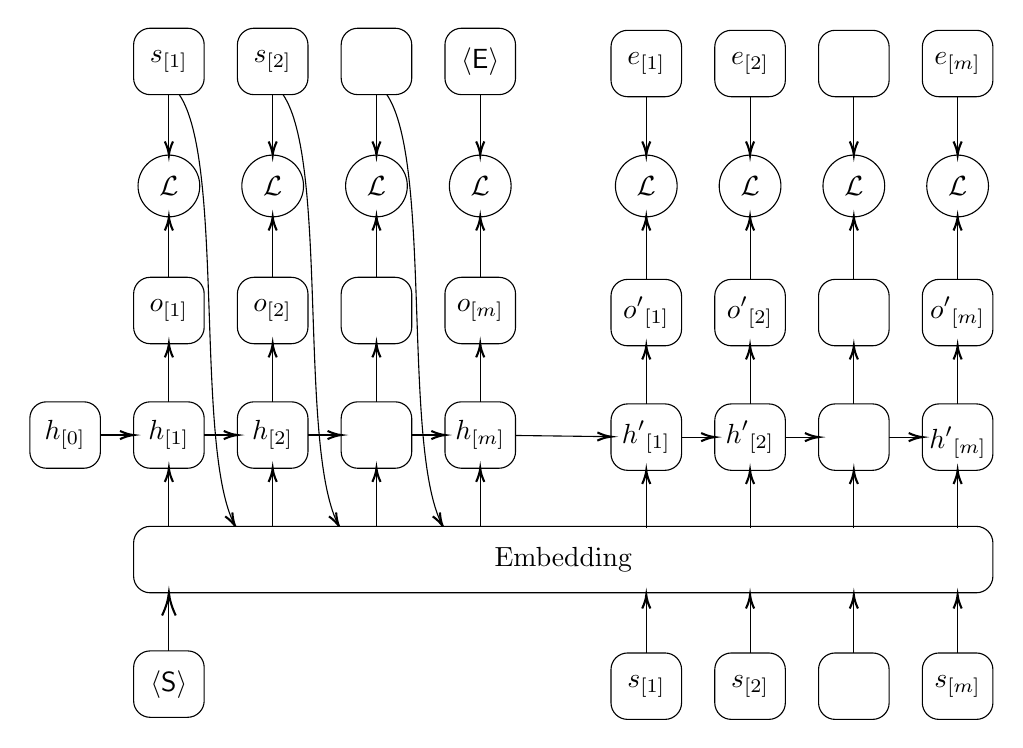
\begin{tikzpicture}[x=0.75pt,y=0.75pt,yscale=-1,xscale=1]
%uncomment if require: \path (0,400); %set diagram left start at 0, and has height of 400

%Curve Lines [id:da14509372882198068]
\draw    (100,62) .. controls (121.77,94.16) and (107.54,229.5) .. (126.13,268.3) ;
\draw [shift={(127,270)}, rotate = 241.3] [color={rgb, 255:red, 0; green, 0; blue, 0 }  ][line width=0.75]    (6.56,-1.97) .. controls (4.17,-0.84) and (1.99,-0.18) .. (0,0) .. controls (1.99,0.18) and (4.17,0.84) .. (6.56,1.97)   ;
%Curve Lines [id:da32690755901594937]
\draw    (150,62) .. controls (171.77,94.16) and (157.54,229.5) .. (176.13,268.3) ;
\draw [shift={(177,270)}, rotate = 241.3] [color={rgb, 255:red, 0; green, 0; blue, 0 }  ][line width=0.75]    (6.56,-1.97) .. controls (4.17,-0.84) and (1.99,-0.18) .. (0,0) .. controls (1.99,0.18) and (4.17,0.84) .. (6.56,1.97)   ;
%Curve Lines [id:da8801757764435838]
\draw    (200,62) .. controls (221.77,94.16) and (207.54,229.5) .. (226.13,268.3) ;
\draw [shift={(227,270)}, rotate = 241.3] [color={rgb, 255:red, 0; green, 0; blue, 0 }  ][line width=0.75]    (6.56,-1.97) .. controls (4.17,-0.84) and (1.99,-0.18) .. (0,0) .. controls (1.99,0.18) and (4.17,0.84) .. (6.56,1.97)   ;

% Text Node
\draw  [fill={rgb, 255:red, 255; green, 255; blue, 255 }  ,fill opacity=1 ]  (78,278) .. controls (78,273.58) and (81.58,270) .. (86,270) -- (484,270) .. controls (488.42,270) and (492,273.58) .. (492,278) -- (492,294) .. controls (492,298.42) and (488.42,302) .. (484,302) -- (86,302) .. controls (81.58,302) and (78,298.42) .. (78,294) -- cycle  ;
\draw (285,286) node   [align=left] {\begin{minipage}[lt]{278.8pt}\setlength\topsep{0pt}
\begin{center}
Embedding
\end{center}

\end{minipage}};
% Text Node
\draw (95,286) node   [align=left] {\begin{minipage}[lt]{20.400000000000002pt}\setlength\topsep{0pt}
\begin{center}
\end{center}

\end{minipage}};
% Text Node
\draw (145,286) node   [align=left] {\begin{minipage}[lt]{20.400000000000002pt}\setlength\topsep{0pt}
\begin{center}
\end{center}

\end{minipage}};
% Text Node
\draw (195,286) node   [align=left] {\begin{minipage}[lt]{20.400000000000002pt}\setlength\topsep{0pt}
\begin{center}
\end{center}

\end{minipage}};
% Text Node
\draw (245,286) node   [align=left] {\begin{minipage}[lt]{20.400000000000002pt}\setlength\topsep{0pt}
\begin{center}
\end{center}

\end{minipage}};
% Text Node
\draw    (78,218) .. controls (78,213.58) and (81.58,210) .. (86,210) -- (104,210) .. controls (108.42,210) and (112,213.58) .. (112,218) -- (112,234) .. controls (112,238.42) and (108.42,242) .. (104,242) -- (86,242) .. controls (81.58,242) and (78,238.42) .. (78,234) -- cycle  ;
\draw (95,226) node   [align=left] {\begin{minipage}[lt]{20.400000000000002pt}\setlength\topsep{0pt}
\begin{center}
$\displaystyle \boldsymbol{h}_{[ 1]}$
\end{center}

\end{minipage}};
% Text Node
\draw    (128,218) .. controls (128,213.58) and (131.58,210) .. (136,210) -- (154,210) .. controls (158.42,210) and (162,213.58) .. (162,218) -- (162,234) .. controls (162,238.42) and (158.42,242) .. (154,242) -- (136,242) .. controls (131.58,242) and (128,238.42) .. (128,234) -- cycle  ;
\draw (145,226) node   [align=left] {\begin{minipage}[lt]{20.400000000000002pt}\setlength\topsep{0pt}
\begin{center}
$\displaystyle \boldsymbol{h}_{[ 2]}$
\end{center}

\end{minipage}};
% Text Node
\draw    (178,218) .. controls (178,213.58) and (181.58,210) .. (186,210) -- (204,210) .. controls (208.42,210) and (212,213.58) .. (212,218) -- (212,234) .. controls (212,238.42) and (208.42,242) .. (204,242) -- (186,242) .. controls (181.58,242) and (178,238.42) .. (178,234) -- cycle  ;
\draw (195,226) node   [align=left] {\begin{minipage}[lt]{20.400000000000002pt}\setlength\topsep{0pt}
\begin{center}
$\displaystyle \dotsc $
\end{center}

\end{minipage}};
% Text Node
\draw    (228,218) .. controls (228,213.58) and (231.58,210) .. (236,210) -- (254,210) .. controls (258.42,210) and (262,213.58) .. (262,218) -- (262,234) .. controls (262,238.42) and (258.42,242) .. (254,242) -- (236,242) .. controls (231.58,242) and (228,238.42) .. (228,234) -- cycle  ;
\draw (245,226) node   [align=left] {\begin{minipage}[lt]{20.400000000000002pt}\setlength\topsep{0pt}
\begin{center}
$\displaystyle \boldsymbol{h}_{[ m]}$
\end{center}

\end{minipage}};
% Text Node
\draw    (78,158) .. controls (78,153.58) and (81.58,150) .. (86,150) -- (104,150) .. controls (108.42,150) and (112,153.58) .. (112,158) -- (112,174) .. controls (112,178.42) and (108.42,182) .. (104,182) -- (86,182) .. controls (81.58,182) and (78,178.42) .. (78,174) -- cycle  ;
\draw (95,166) node   [align=left] {\begin{minipage}[lt]{20.400000000000002pt}\setlength\topsep{0pt}
\begin{center}
$\displaystyle \boldsymbol{o}_{[ 1]}$
\end{center}

\end{minipage}};
% Text Node
\draw    (128,158) .. controls (128,153.58) and (131.58,150) .. (136,150) -- (154,150) .. controls (158.42,150) and (162,153.58) .. (162,158) -- (162,174) .. controls (162,178.42) and (158.42,182) .. (154,182) -- (136,182) .. controls (131.58,182) and (128,178.42) .. (128,174) -- cycle  ;
\draw (145,166) node   [align=left] {\begin{minipage}[lt]{20.400000000000002pt}\setlength\topsep{0pt}
\begin{center}
$\displaystyle \boldsymbol{o}_{[ 2]}$
\end{center}

\end{minipage}};
% Text Node
\draw    (178,158) .. controls (178,153.58) and (181.58,150) .. (186,150) -- (204,150) .. controls (208.42,150) and (212,153.58) .. (212,158) -- (212,174) .. controls (212,178.42) and (208.42,182) .. (204,182) -- (186,182) .. controls (181.58,182) and (178,178.42) .. (178,174) -- cycle  ;
\draw (195,166) node   [align=left] {\begin{minipage}[lt]{20.400000000000002pt}\setlength\topsep{0pt}
\begin{center}
$\displaystyle \dotsc $
\end{center}

\end{minipage}};
% Text Node
\draw    (228,158) .. controls (228,153.58) and (231.58,150) .. (236,150) -- (254,150) .. controls (258.42,150) and (262,153.58) .. (262,158) -- (262,174) .. controls (262,178.42) and (258.42,182) .. (254,182) -- (236,182) .. controls (231.58,182) and (228,178.42) .. (228,174) -- cycle  ;
\draw (245,166) node   [align=left] {\begin{minipage}[lt]{20.400000000000002pt}\setlength\topsep{0pt}
\begin{center}
$\displaystyle \boldsymbol{o}_{[ m]}$
\end{center}

\end{minipage}};
% Text Node
\draw    (308,339) .. controls (308,334.58) and (311.58,331) .. (316,331) -- (334,331) .. controls (338.42,331) and (342,334.58) .. (342,339) -- (342,355) .. controls (342,359.42) and (338.42,363) .. (334,363) -- (316,363) .. controls (311.58,363) and (308,359.42) .. (308,355) -- cycle  ;
\draw (325,347) node   [align=left] {\begin{minipage}[lt]{20.400000000000002pt}\setlength\topsep{0pt}
\begin{center}
$\displaystyle \boldsymbol{s}_{[ 1]}$
\end{center}

\end{minipage}};
% Text Node
\draw (325,287) node   [align=left] {\begin{minipage}[lt]{20.400000000000002pt}\setlength\topsep{0pt}
\begin{center}
\end{center}

\end{minipage}};
% Text Node
\draw    (358,339) .. controls (358,334.58) and (361.58,331) .. (366,331) -- (384,331) .. controls (388.42,331) and (392,334.58) .. (392,339) -- (392,355) .. controls (392,359.42) and (388.42,363) .. (384,363) -- (366,363) .. controls (361.58,363) and (358,359.42) .. (358,355) -- cycle  ;
\draw (375,347) node   [align=left] {\begin{minipage}[lt]{20.400000000000002pt}\setlength\topsep{0pt}
\begin{center}
$\displaystyle \boldsymbol{s}_{[ 2]}$
\end{center}

\end{minipage}};
% Text Node
\draw    (408,339) .. controls (408,334.58) and (411.58,331) .. (416,331) -- (434,331) .. controls (438.42,331) and (442,334.58) .. (442,339) -- (442,355) .. controls (442,359.42) and (438.42,363) .. (434,363) -- (416,363) .. controls (411.58,363) and (408,359.42) .. (408,355) -- cycle  ;
\draw (425,347) node   [align=left] {\begin{minipage}[lt]{20.400000000000002pt}\setlength\topsep{0pt}
\begin{center}
$\displaystyle \dotsc $
\end{center}

\end{minipage}};
% Text Node
\draw    (458,339) .. controls (458,334.58) and (461.58,331) .. (466,331) -- (484,331) .. controls (488.42,331) and (492,334.58) .. (492,339) -- (492,355) .. controls (492,359.42) and (488.42,363) .. (484,363) -- (466,363) .. controls (461.58,363) and (458,359.42) .. (458,355) -- cycle  ;
\draw (475,347) node   [align=left] {\begin{minipage}[lt]{20.400000000000002pt}\setlength\topsep{0pt}
\begin{center}
$\displaystyle \boldsymbol{s}_{[ m]}$
\end{center}

\end{minipage}};
% Text Node
\draw (375,287) node   [align=left] {\begin{minipage}[lt]{20.400000000000002pt}\setlength\topsep{0pt}
\begin{center}
\end{center}

\end{minipage}};
% Text Node
\draw (425,287) node   [align=left] {\begin{minipage}[lt]{20.400000000000002pt}\setlength\topsep{0pt}
\begin{center}
\end{center}

\end{minipage}};
% Text Node
\draw (475,287) node   [align=left] {\begin{minipage}[lt]{20.400000000000002pt}\setlength\topsep{0pt}
\begin{center}
\end{center}

\end{minipage}};
% Text Node
\draw    (308,219) .. controls (308,214.58) and (311.58,211) .. (316,211) -- (334,211) .. controls (338.42,211) and (342,214.58) .. (342,219) -- (342,235) .. controls (342,239.42) and (338.42,243) .. (334,243) -- (316,243) .. controls (311.58,243) and (308,239.42) .. (308,235) -- cycle  ;
\draw (325,227) node   [align=left] {\begin{minipage}[lt]{20.400000000000002pt}\setlength\topsep{0pt}
\begin{center}
$\displaystyle \boldsymbol{h'}_{[ 1]}$
\end{center}

\end{minipage}};
% Text Node
\draw    (358,219) .. controls (358,214.58) and (361.58,211) .. (366,211) -- (384,211) .. controls (388.42,211) and (392,214.58) .. (392,219) -- (392,235) .. controls (392,239.42) and (388.42,243) .. (384,243) -- (366,243) .. controls (361.58,243) and (358,239.42) .. (358,235) -- cycle  ;
\draw (375,227) node   [align=left] {\begin{minipage}[lt]{20.400000000000002pt}\setlength\topsep{0pt}
\begin{center}
$\displaystyle \boldsymbol{h'}_{[ 2]}$
\end{center}

\end{minipage}};
% Text Node
\draw    (408,219) .. controls (408,214.58) and (411.58,211) .. (416,211) -- (434,211) .. controls (438.42,211) and (442,214.58) .. (442,219) -- (442,235) .. controls (442,239.42) and (438.42,243) .. (434,243) -- (416,243) .. controls (411.58,243) and (408,239.42) .. (408,235) -- cycle  ;
\draw (425,227) node   [align=left] {\begin{minipage}[lt]{20.400000000000002pt}\setlength\topsep{0pt}
\begin{center}
$\displaystyle \dotsc $
\end{center}

\end{minipage}};
% Text Node
\draw    (458,219) .. controls (458,214.58) and (461.58,211) .. (466,211) -- (484,211) .. controls (488.42,211) and (492,214.58) .. (492,219) -- (492,235) .. controls (492,239.42) and (488.42,243) .. (484,243) -- (466,243) .. controls (461.58,243) and (458,239.42) .. (458,235) -- cycle  ;
\draw (475,227) node   [align=left] {\begin{minipage}[lt]{20.400000000000002pt}\setlength\topsep{0pt}
\begin{center}
$\displaystyle \boldsymbol{h'}_{[ m]}$
\end{center}

\end{minipage}};
% Text Node
\draw    (308,159) .. controls (308,154.58) and (311.58,151) .. (316,151) -- (334,151) .. controls (338.42,151) and (342,154.58) .. (342,159) -- (342,175) .. controls (342,179.42) and (338.42,183) .. (334,183) -- (316,183) .. controls (311.58,183) and (308,179.42) .. (308,175) -- cycle  ;
\draw (325,167) node   [align=left] {\begin{minipage}[lt]{20.400000000000002pt}\setlength\topsep{0pt}
\begin{center}
$\displaystyle \boldsymbol{o'}_{[ 1]}$
\end{center}

\end{minipage}};
% Text Node
\draw    (358,159) .. controls (358,154.58) and (361.58,151) .. (366,151) -- (384,151) .. controls (388.42,151) and (392,154.58) .. (392,159) -- (392,175) .. controls (392,179.42) and (388.42,183) .. (384,183) -- (366,183) .. controls (361.58,183) and (358,179.42) .. (358,175) -- cycle  ;
\draw (375,167) node   [align=left] {\begin{minipage}[lt]{20.400000000000002pt}\setlength\topsep{0pt}
\begin{center}
$\displaystyle \boldsymbol{o'}_{[ 2]}$
\end{center}

\end{minipage}};
% Text Node
\draw    (408,159) .. controls (408,154.58) and (411.58,151) .. (416,151) -- (434,151) .. controls (438.42,151) and (442,154.58) .. (442,159) -- (442,175) .. controls (442,179.42) and (438.42,183) .. (434,183) -- (416,183) .. controls (411.58,183) and (408,179.42) .. (408,175) -- cycle  ;
\draw (425,167) node   [align=left] {\begin{minipage}[lt]{20.400000000000002pt}\setlength\topsep{0pt}
\begin{center}
$\displaystyle \dotsc $
\end{center}

\end{minipage}};
% Text Node
\draw    (458,159) .. controls (458,154.58) and (461.58,151) .. (466,151) -- (484,151) .. controls (488.42,151) and (492,154.58) .. (492,159) -- (492,175) .. controls (492,179.42) and (488.42,183) .. (484,183) -- (466,183) .. controls (461.58,183) and (458,179.42) .. (458,175) -- cycle  ;
\draw (475,167) node   [align=left] {\begin{minipage}[lt]{20.400000000000002pt}\setlength\topsep{0pt}
\begin{center}
$\displaystyle \boldsymbol{o'}_{[ m]}$
\end{center}

\end{minipage}};
% Text Node
\draw    (95, 106) circle [x radius= 14.87, y radius= 14.87]   ;
\draw (95,106) node   [align=left] {\begin{minipage}[lt]{13.600000000000001pt}\setlength\topsep{0pt}
\begin{center}
$\displaystyle \mathcal{L}$
\end{center}

\end{minipage}};
% Text Node
\draw    (145, 106) circle [x radius= 14.87, y radius= 14.87]   ;
\draw (145,106) node   [align=left] {\begin{minipage}[lt]{13.600000000000001pt}\setlength\topsep{0pt}
\begin{center}
$\displaystyle \mathcal{L}$
\end{center}

\end{minipage}};
% Text Node
\draw    (195, 106) circle [x radius= 14.87, y radius= 14.87]   ;
\draw (195,106) node   [align=left] {\begin{minipage}[lt]{13.600000000000001pt}\setlength\topsep{0pt}
\begin{center}
$\displaystyle \mathcal{L}$
\end{center}

\end{minipage}};
% Text Node
\draw    (245, 106) circle [x radius= 14.87, y radius= 14.87]   ;
\draw (245,106) node   [align=left] {\begin{minipage}[lt]{13.600000000000001pt}\setlength\topsep{0pt}
\begin{center}
$\displaystyle \mathcal{L}$
\end{center}

\end{minipage}};
% Text Node
\draw    (325, 106) circle [x radius= 14.87, y radius= 14.87]   ;
\draw (325,106) node   [align=left] {\begin{minipage}[lt]{13.600000000000001pt}\setlength\topsep{0pt}
\begin{center}
$\displaystyle \mathcal{L}$
\end{center}

\end{minipage}};
% Text Node
\draw    (375, 106) circle [x radius= 14.87, y radius= 14.87]   ;
\draw (375,106) node   [align=left] {\begin{minipage}[lt]{13.600000000000001pt}\setlength\topsep{0pt}
\begin{center}
$\displaystyle \mathcal{L}$
\end{center}

\end{minipage}};
% Text Node
\draw    (425, 106) circle [x radius= 14.87, y radius= 14.87]   ;
\draw (425,106) node   [align=left] {\begin{minipage}[lt]{13.600000000000001pt}\setlength\topsep{0pt}
\begin{center}
$\displaystyle \mathcal{L}$
\end{center}

\end{minipage}};
% Text Node
\draw    (475, 106) circle [x radius= 14.87, y radius= 14.87]   ;
\draw (475,106) node   [align=left] {\begin{minipage}[lt]{13.600000000000001pt}\setlength\topsep{0pt}
\begin{center}
$\displaystyle \mathcal{L}$
\end{center}

\end{minipage}};
% Text Node
\draw    (78,38) .. controls (78,33.58) and (81.58,30) .. (86,30) -- (104,30) .. controls (108.42,30) and (112,33.58) .. (112,38) -- (112,54) .. controls (112,58.42) and (108.42,62) .. (104,62) -- (86,62) .. controls (81.58,62) and (78,58.42) .. (78,54) -- cycle  ;
\draw (95,46) node   [align=left] {\begin{minipage}[lt]{20.400000000000002pt}\setlength\topsep{0pt}
\begin{center}
$\displaystyle \boldsymbol{s}_{[ 1]}$
\end{center}

\end{minipage}};
% Text Node
\draw    (128,38) .. controls (128,33.58) and (131.58,30) .. (136,30) -- (154,30) .. controls (158.42,30) and (162,33.58) .. (162,38) -- (162,54) .. controls (162,58.42) and (158.42,62) .. (154,62) -- (136,62) .. controls (131.58,62) and (128,58.42) .. (128,54) -- cycle  ;
\draw (145,46) node   [align=left] {\begin{minipage}[lt]{20.400000000000002pt}\setlength\topsep{0pt}
\begin{center}
$\displaystyle \boldsymbol{s}_{[ 2]}$
\end{center}

\end{minipage}};
% Text Node
\draw    (178,38) .. controls (178,33.58) and (181.58,30) .. (186,30) -- (204,30) .. controls (208.42,30) and (212,33.58) .. (212,38) -- (212,54) .. controls (212,58.42) and (208.42,62) .. (204,62) -- (186,62) .. controls (181.58,62) and (178,58.42) .. (178,54) -- cycle  ;
\draw (195,46) node   [align=left] {\begin{minipage}[lt]{20.400000000000002pt}\setlength\topsep{0pt}
\begin{center}
$\displaystyle \dotsc $
\end{center}

\end{minipage}};
% Text Node
\draw    (228,38) .. controls (228,33.58) and (231.58,30) .. (236,30) -- (254,30) .. controls (258.42,30) and (262,33.58) .. (262,38) -- (262,54) .. controls (262,58.42) and (258.42,62) .. (254,62) -- (236,62) .. controls (231.58,62) and (228,58.42) .. (228,54) -- cycle  ;
\draw (245,46) node   [align=left] {\begin{minipage}[lt]{20.400000000000002pt}\setlength\topsep{0pt}
\begin{center}
$\displaystyle \langle \mathsf{E} \rangle $
\end{center}

\end{minipage}};
% Text Node
\draw    (308,39) .. controls (308,34.58) and (311.58,31) .. (316,31) -- (334,31) .. controls (338.42,31) and (342,34.58) .. (342,39) -- (342,55) .. controls (342,59.42) and (338.42,63) .. (334,63) -- (316,63) .. controls (311.58,63) and (308,59.42) .. (308,55) -- cycle  ;
\draw (325,47) node   [align=left] {\begin{minipage}[lt]{20.400000000000002pt}\setlength\topsep{0pt}
\begin{center}
$\displaystyle \boldsymbol{e}_{[ 1]}$
\end{center}

\end{minipage}};
% Text Node
\draw    (358,39) .. controls (358,34.58) and (361.58,31) .. (366,31) -- (384,31) .. controls (388.42,31) and (392,34.58) .. (392,39) -- (392,55) .. controls (392,59.42) and (388.42,63) .. (384,63) -- (366,63) .. controls (361.58,63) and (358,59.42) .. (358,55) -- cycle  ;
\draw (375,47) node   [align=left] {\begin{minipage}[lt]{20.400000000000002pt}\setlength\topsep{0pt}
\begin{center}
$\displaystyle \boldsymbol{e}_{[ 2]}$
\end{center}

\end{minipage}};
% Text Node
\draw    (408,39) .. controls (408,34.58) and (411.58,31) .. (416,31) -- (434,31) .. controls (438.42,31) and (442,34.58) .. (442,39) -- (442,55) .. controls (442,59.42) and (438.42,63) .. (434,63) -- (416,63) .. controls (411.58,63) and (408,59.42) .. (408,55) -- cycle  ;
\draw (425,47) node   [align=left] {\begin{minipage}[lt]{20.400000000000002pt}\setlength\topsep{0pt}
\begin{center}
$\displaystyle \dotsc $
\end{center}

\end{minipage}};
% Text Node
\draw    (458,39) .. controls (458,34.58) and (461.58,31) .. (466,31) -- (484,31) .. controls (488.42,31) and (492,34.58) .. (492,39) -- (492,55) .. controls (492,59.42) and (488.42,63) .. (484,63) -- (466,63) .. controls (461.58,63) and (458,59.42) .. (458,55) -- cycle  ;
\draw (475,47) node   [align=left] {\begin{minipage}[lt]{20.400000000000002pt}\setlength\topsep{0pt}
\begin{center}
$\displaystyle \boldsymbol{e}_{[ m]}$
\end{center}

\end{minipage}};
% Text Node
\draw    (28,218) .. controls (28,213.58) and (31.58,210) .. (36,210) -- (54,210) .. controls (58.42,210) and (62,213.58) .. (62,218) -- (62,234) .. controls (62,238.42) and (58.42,242) .. (54,242) -- (36,242) .. controls (31.58,242) and (28,238.42) .. (28,234) -- cycle  ;
\draw (45,226) node   [align=left] {\begin{minipage}[lt]{20.400000000000002pt}\setlength\topsep{0pt}
\begin{center}
$\displaystyle \boldsymbol{h}_{[ 0]}$
\end{center}

\end{minipage}};
% Text Node
\draw    (78,338) .. controls (78,333.58) and (81.58,330) .. (86,330) -- (104,330) .. controls (108.42,330) and (112,333.58) .. (112,338) -- (112,354) .. controls (112,358.42) and (108.42,362) .. (104,362) -- (86,362) .. controls (81.58,362) and (78,358.42) .. (78,354) -- cycle  ;
\draw (95,346) node   [align=left] {\begin{minipage}[lt]{20.400000000000002pt}\setlength\topsep{0pt}
\begin{center}
$\displaystyle \langle \mathsf{S} \rangle $
\end{center}

\end{minipage}};
% Connection
\draw    (325,331) -- (325,305) ;
\draw [shift={(325,303)}, rotate = 450] [color={rgb, 255:red, 0; green, 0; blue, 0 }  ][line width=0.75]    (6.56,-1.97) .. controls (4.17,-0.84) and (1.99,-0.18) .. (0,0) .. controls (1.99,0.18) and (4.17,0.84) .. (6.56,1.97)   ;
% Connection
\draw    (375,331) -- (375,305) ;
\draw [shift={(375,303)}, rotate = 450] [color={rgb, 255:red, 0; green, 0; blue, 0 }  ][line width=0.75]    (6.56,-1.97) .. controls (4.17,-0.84) and (1.99,-0.18) .. (0,0) .. controls (1.99,0.18) and (4.17,0.84) .. (6.56,1.97)   ;
% Connection
\draw    (425,331) -- (425,305) ;
\draw [shift={(425,303)}, rotate = 450] [color={rgb, 255:red, 0; green, 0; blue, 0 }  ][line width=0.75]    (6.56,-1.97) .. controls (4.17,-0.84) and (1.99,-0.18) .. (0,0) .. controls (1.99,0.18) and (4.17,0.84) .. (6.56,1.97)   ;
% Connection
\draw    (475,331) -- (475,305) ;
\draw [shift={(475,303)}, rotate = 450] [color={rgb, 255:red, 0; green, 0; blue, 0 }  ][line width=0.75]    (6.56,-1.97) .. controls (4.17,-0.84) and (1.99,-0.18) .. (0,0) .. controls (1.99,0.18) and (4.17,0.84) .. (6.56,1.97)   ;
% Connection
\draw    (95,270) -- (95,244) ;
\draw [shift={(95,242)}, rotate = 450] [color={rgb, 255:red, 0; green, 0; blue, 0 }  ][line width=0.75]    (6.56,-1.97) .. controls (4.17,-0.84) and (1.99,-0.18) .. (0,0) .. controls (1.99,0.18) and (4.17,0.84) .. (6.56,1.97)   ;
% Connection
\draw    (145,270) -- (145,244) ;
\draw [shift={(145,242)}, rotate = 450] [color={rgb, 255:red, 0; green, 0; blue, 0 }  ][line width=0.75]    (6.56,-1.97) .. controls (4.17,-0.84) and (1.99,-0.18) .. (0,0) .. controls (1.99,0.18) and (4.17,0.84) .. (6.56,1.97)   ;
% Connection
\draw    (195,270) -- (195,244) ;
\draw [shift={(195,242)}, rotate = 450] [color={rgb, 255:red, 0; green, 0; blue, 0 }  ][line width=0.75]    (6.56,-1.97) .. controls (4.17,-0.84) and (1.99,-0.18) .. (0,0) .. controls (1.99,0.18) and (4.17,0.84) .. (6.56,1.97)   ;
% Connection
\draw    (245,270) -- (245,244) ;
\draw [shift={(245,242)}, rotate = 450] [color={rgb, 255:red, 0; green, 0; blue, 0 }  ][line width=0.75]    (6.56,-1.97) .. controls (4.17,-0.84) and (1.99,-0.18) .. (0,0) .. controls (1.99,0.18) and (4.17,0.84) .. (6.56,1.97)   ;
% Connection
\draw    (325,271) -- (325,245) ;
\draw [shift={(325,243)}, rotate = 450] [color={rgb, 255:red, 0; green, 0; blue, 0 }  ][line width=0.75]    (6.56,-1.97) .. controls (4.17,-0.84) and (1.99,-0.18) .. (0,0) .. controls (1.99,0.18) and (4.17,0.84) .. (6.56,1.97)   ;
% Connection
\draw    (375,271) -- (375,245) ;
\draw [shift={(375,243)}, rotate = 450] [color={rgb, 255:red, 0; green, 0; blue, 0 }  ][line width=0.75]    (6.56,-1.97) .. controls (4.17,-0.84) and (1.99,-0.18) .. (0,0) .. controls (1.99,0.18) and (4.17,0.84) .. (6.56,1.97)   ;
% Connection
\draw    (425,271) -- (425,245) ;
\draw [shift={(425,243)}, rotate = 450] [color={rgb, 255:red, 0; green, 0; blue, 0 }  ][line width=0.75]    (6.56,-1.97) .. controls (4.17,-0.84) and (1.99,-0.18) .. (0,0) .. controls (1.99,0.18) and (4.17,0.84) .. (6.56,1.97)   ;
% Connection
\draw    (475,271) -- (475,245) ;
\draw [shift={(475,243)}, rotate = 450] [color={rgb, 255:red, 0; green, 0; blue, 0 }  ][line width=0.75]    (6.56,-1.97) .. controls (4.17,-0.84) and (1.99,-0.18) .. (0,0) .. controls (1.99,0.18) and (4.17,0.84) .. (6.56,1.97)   ;
% Connection
\draw    (112,226) -- (126,226) ;
\draw [shift={(128,226)}, rotate = 180] [color={rgb, 255:red, 0; green, 0; blue, 0 }  ][line width=0.75]    (6.56,-1.97) .. controls (4.17,-0.84) and (1.99,-0.18) .. (0,0) .. controls (1.99,0.18) and (4.17,0.84) .. (6.56,1.97)   ;
% Connection
\draw    (162,226) -- (176,226) ;
\draw [shift={(178,226)}, rotate = 180] [color={rgb, 255:red, 0; green, 0; blue, 0 }  ][line width=0.75]    (6.56,-1.97) .. controls (4.17,-0.84) and (1.99,-0.18) .. (0,0) .. controls (1.99,0.18) and (4.17,0.84) .. (6.56,1.97)   ;
% Connection
\draw    (212,226) -- (226,226) ;
\draw [shift={(228,226)}, rotate = 180] [color={rgb, 255:red, 0; green, 0; blue, 0 }  ][line width=0.75]    (6.56,-1.97) .. controls (4.17,-0.84) and (1.99,-0.18) .. (0,0) .. controls (1.99,0.18) and (4.17,0.84) .. (6.56,1.97)   ;
% Connection
\draw    (262,226.21) -- (306,226.76) ;
\draw [shift={(308,226.79)}, rotate = 180.72] [color={rgb, 255:red, 0; green, 0; blue, 0 }  ][line width=0.75]    (6.56,-1.97) .. controls (4.17,-0.84) and (1.99,-0.18) .. (0,0) .. controls (1.99,0.18) and (4.17,0.84) .. (6.56,1.97)   ;
% Connection
\draw    (342,227) -- (356,227) ;
\draw [shift={(358,227)}, rotate = 180] [color={rgb, 255:red, 0; green, 0; blue, 0 }  ][line width=0.75]    (6.56,-1.97) .. controls (4.17,-0.84) and (1.99,-0.18) .. (0,0) .. controls (1.99,0.18) and (4.17,0.84) .. (6.56,1.97)   ;
% Connection
\draw    (392,227) -- (406,227) ;
\draw [shift={(408,227)}, rotate = 180] [color={rgb, 255:red, 0; green, 0; blue, 0 }  ][line width=0.75]    (6.56,-1.97) .. controls (4.17,-0.84) and (1.99,-0.18) .. (0,0) .. controls (1.99,0.18) and (4.17,0.84) .. (6.56,1.97)   ;
% Connection
\draw    (442,227) -- (456,227) ;
\draw [shift={(458,227)}, rotate = 180] [color={rgb, 255:red, 0; green, 0; blue, 0 }  ][line width=0.75]    (6.56,-1.97) .. controls (4.17,-0.84) and (1.99,-0.18) .. (0,0) .. controls (1.99,0.18) and (4.17,0.84) .. (6.56,1.97)   ;
% Connection
\draw    (95,210) -- (95,184) ;
\draw [shift={(95,182)}, rotate = 450] [color={rgb, 255:red, 0; green, 0; blue, 0 }  ][line width=0.75]    (6.56,-1.97) .. controls (4.17,-0.84) and (1.99,-0.18) .. (0,0) .. controls (1.99,0.18) and (4.17,0.84) .. (6.56,1.97)   ;
% Connection
\draw    (145,210) -- (145,184) ;
\draw [shift={(145,182)}, rotate = 450] [color={rgb, 255:red, 0; green, 0; blue, 0 }  ][line width=0.75]    (6.56,-1.97) .. controls (4.17,-0.84) and (1.99,-0.18) .. (0,0) .. controls (1.99,0.18) and (4.17,0.84) .. (6.56,1.97)   ;
% Connection
\draw    (195,210) -- (195,184) ;
\draw [shift={(195,182)}, rotate = 450] [color={rgb, 255:red, 0; green, 0; blue, 0 }  ][line width=0.75]    (6.56,-1.97) .. controls (4.17,-0.84) and (1.99,-0.18) .. (0,0) .. controls (1.99,0.18) and (4.17,0.84) .. (6.56,1.97)   ;
% Connection
\draw    (245,210) -- (245,184) ;
\draw [shift={(245,182)}, rotate = 450] [color={rgb, 255:red, 0; green, 0; blue, 0 }  ][line width=0.75]    (6.56,-1.97) .. controls (4.17,-0.84) and (1.99,-0.18) .. (0,0) .. controls (1.99,0.18) and (4.17,0.84) .. (6.56,1.97)   ;
% Connection
\draw    (325,211) -- (325,185) ;
\draw [shift={(325,183)}, rotate = 450] [color={rgb, 255:red, 0; green, 0; blue, 0 }  ][line width=0.75]    (6.56,-1.97) .. controls (4.17,-0.84) and (1.99,-0.18) .. (0,0) .. controls (1.99,0.18) and (4.17,0.84) .. (6.56,1.97)   ;
% Connection
\draw    (375,211) -- (375,185) ;
\draw [shift={(375,183)}, rotate = 450] [color={rgb, 255:red, 0; green, 0; blue, 0 }  ][line width=0.75]    (6.56,-1.97) .. controls (4.17,-0.84) and (1.99,-0.18) .. (0,0) .. controls (1.99,0.18) and (4.17,0.84) .. (6.56,1.97)   ;
% Connection
\draw    (425,211) -- (425,185) ;
\draw [shift={(425,183)}, rotate = 450] [color={rgb, 255:red, 0; green, 0; blue, 0 }  ][line width=0.75]    (6.56,-1.97) .. controls (4.17,-0.84) and (1.99,-0.18) .. (0,0) .. controls (1.99,0.18) and (4.17,0.84) .. (6.56,1.97)   ;
% Connection
\draw    (475,211) -- (475,185) ;
\draw [shift={(475,183)}, rotate = 450] [color={rgb, 255:red, 0; green, 0; blue, 0 }  ][line width=0.75]    (6.56,-1.97) .. controls (4.17,-0.84) and (1.99,-0.18) .. (0,0) .. controls (1.99,0.18) and (4.17,0.84) .. (6.56,1.97)   ;
% Connection
\draw    (95,150) -- (95,122.87) ;
\draw [shift={(95,120.87)}, rotate = 450] [color={rgb, 255:red, 0; green, 0; blue, 0 }  ][line width=0.75]    (6.56,-1.97) .. controls (4.17,-0.84) and (1.99,-0.18) .. (0,0) .. controls (1.99,0.18) and (4.17,0.84) .. (6.56,1.97)   ;
% Connection
\draw    (145,150) -- (145,122.87) ;
\draw [shift={(145,120.87)}, rotate = 450] [color={rgb, 255:red, 0; green, 0; blue, 0 }  ][line width=0.75]    (6.56,-1.97) .. controls (4.17,-0.84) and (1.99,-0.18) .. (0,0) .. controls (1.99,0.18) and (4.17,0.84) .. (6.56,1.97)   ;
% Connection
\draw    (195,150) -- (195,122.87) ;
\draw [shift={(195,120.87)}, rotate = 450] [color={rgb, 255:red, 0; green, 0; blue, 0 }  ][line width=0.75]    (6.56,-1.97) .. controls (4.17,-0.84) and (1.99,-0.18) .. (0,0) .. controls (1.99,0.18) and (4.17,0.84) .. (6.56,1.97)   ;
% Connection
\draw    (245,150) -- (245,122.87) ;
\draw [shift={(245,120.87)}, rotate = 450] [color={rgb, 255:red, 0; green, 0; blue, 0 }  ][line width=0.75]    (6.56,-1.97) .. controls (4.17,-0.84) and (1.99,-0.18) .. (0,0) .. controls (1.99,0.18) and (4.17,0.84) .. (6.56,1.97)   ;
% Connection
\draw    (325,151) -- (325,122.87) ;
\draw [shift={(325,120.87)}, rotate = 450] [color={rgb, 255:red, 0; green, 0; blue, 0 }  ][line width=0.75]    (6.56,-1.97) .. controls (4.17,-0.84) and (1.99,-0.18) .. (0,0) .. controls (1.99,0.18) and (4.17,0.84) .. (6.56,1.97)   ;
% Connection
\draw    (375,151) -- (375,122.87) ;
\draw [shift={(375,120.87)}, rotate = 450] [color={rgb, 255:red, 0; green, 0; blue, 0 }  ][line width=0.75]    (6.56,-1.97) .. controls (4.17,-0.84) and (1.99,-0.18) .. (0,0) .. controls (1.99,0.18) and (4.17,0.84) .. (6.56,1.97)   ;
% Connection
\draw    (425,151) -- (425,122.87) ;
\draw [shift={(425,120.87)}, rotate = 450] [color={rgb, 255:red, 0; green, 0; blue, 0 }  ][line width=0.75]    (6.56,-1.97) .. controls (4.17,-0.84) and (1.99,-0.18) .. (0,0) .. controls (1.99,0.18) and (4.17,0.84) .. (6.56,1.97)   ;
% Connection
\draw    (475,151) -- (475,122.87) ;
\draw [shift={(475,120.87)}, rotate = 450] [color={rgb, 255:red, 0; green, 0; blue, 0 }  ][line width=0.75]    (6.56,-1.97) .. controls (4.17,-0.84) and (1.99,-0.18) .. (0,0) .. controls (1.99,0.18) and (4.17,0.84) .. (6.56,1.97)   ;
% Connection
\draw    (95,62) -- (95,89.13) ;
\draw [shift={(95,91.13)}, rotate = 270] [color={rgb, 255:red, 0; green, 0; blue, 0 }  ][line width=0.75]    (6.56,-1.97) .. controls (4.17,-0.84) and (1.99,-0.18) .. (0,0) .. controls (1.99,0.18) and (4.17,0.84) .. (6.56,1.97)   ;
% Connection
\draw    (145,62) -- (145,89.13) ;
\draw [shift={(145,91.13)}, rotate = 270] [color={rgb, 255:red, 0; green, 0; blue, 0 }  ][line width=0.75]    (6.56,-1.97) .. controls (4.17,-0.84) and (1.99,-0.18) .. (0,0) .. controls (1.99,0.18) and (4.17,0.84) .. (6.56,1.97)   ;
% Connection
\draw    (195,62) -- (195,89.13) ;
\draw [shift={(195,91.13)}, rotate = 270] [color={rgb, 255:red, 0; green, 0; blue, 0 }  ][line width=0.75]    (6.56,-1.97) .. controls (4.17,-0.84) and (1.99,-0.18) .. (0,0) .. controls (1.99,0.18) and (4.17,0.84) .. (6.56,1.97)   ;
% Connection
\draw    (245,62) -- (245,89.13) ;
\draw [shift={(245,91.13)}, rotate = 270] [color={rgb, 255:red, 0; green, 0; blue, 0 }  ][line width=0.75]    (6.56,-1.97) .. controls (4.17,-0.84) and (1.99,-0.18) .. (0,0) .. controls (1.99,0.18) and (4.17,0.84) .. (6.56,1.97)   ;
% Connection
\draw    (325,63) -- (325,89.13) ;
\draw [shift={(325,91.13)}, rotate = 270] [color={rgb, 255:red, 0; green, 0; blue, 0 }  ][line width=0.75]    (6.56,-1.97) .. controls (4.17,-0.84) and (1.99,-0.18) .. (0,0) .. controls (1.99,0.18) and (4.17,0.84) .. (6.56,1.97)   ;
% Connection
\draw    (375,63) -- (375,89.13) ;
\draw [shift={(375,91.13)}, rotate = 270] [color={rgb, 255:red, 0; green, 0; blue, 0 }  ][line width=0.75]    (6.56,-1.97) .. controls (4.17,-0.84) and (1.99,-0.18) .. (0,0) .. controls (1.99,0.18) and (4.17,0.84) .. (6.56,1.97)   ;
% Connection
\draw    (425,63) -- (425,89.13) ;
\draw [shift={(425,91.13)}, rotate = 270] [color={rgb, 255:red, 0; green, 0; blue, 0 }  ][line width=0.75]    (6.56,-1.97) .. controls (4.17,-0.84) and (1.99,-0.18) .. (0,0) .. controls (1.99,0.18) and (4.17,0.84) .. (6.56,1.97)   ;
% Connection
\draw    (475,63) -- (475,89.13) ;
\draw [shift={(475,91.13)}, rotate = 270] [color={rgb, 255:red, 0; green, 0; blue, 0 }  ][line width=0.75]    (6.56,-1.97) .. controls (4.17,-0.84) and (1.99,-0.18) .. (0,0) .. controls (1.99,0.18) and (4.17,0.84) .. (6.56,1.97)   ;
% Connection
\draw    (62,226) -- (76,226) ;
\draw [shift={(78,226)}, rotate = 180] [color={rgb, 255:red, 0; green, 0; blue, 0 }  ][line width=0.75]    (6.56,-1.97) .. controls (4.17,-0.84) and (1.99,-0.18) .. (0,0) .. controls (1.99,0.18) and (4.17,0.84) .. (6.56,1.97)   ;
% Connection
\draw    (95,330) -- (95,304) ;
\draw [shift={(95,302)}, rotate = 450] [color={rgb, 255:red, 0; green, 0; blue, 0 }  ][line width=0.75]    (10.93,-3.29) .. controls (6.95,-1.4) and (3.31,-0.3) .. (0,0) .. controls (3.31,0.3) and (6.95,1.4) .. (10.93,3.29)   ;

\end{tikzpicture}}
    \caption{A depiction of the proposed architecture during training. We set $|\tau_S| = |\tau_E| = m$ to avoid cluttering. Notice that the embedding matrix is shared between the two networks.}
    \label{fig:model-training}
\end{figure*}

\subsubsection*{Generation}
To generate an ordered edge sequence, one first generates a starting sequence $\Vector{\tilde{s}}$ from the first network in autoregressive sampling mode. The generative process is started by passing the $\SOS$ token to the network. The categorical distribution corresponding to all the possible Node IDs is sampled at each step, and the resulting node ID is used as input for the next step. The autoregressive sampling is interrupted once the $\EOS$ token is sampled. At this point, the sampled starting sequence $\Vector{\tilde{s}}$ is used as input for the second network, which predicts the ending sequence. This time, the output distribution is not sampled, but the token with the highest probability $\Elem{\hat{e}}{i}$ is chosen at each step. This method is also known as \emph{greedy sampling}, and corresponds to applying the $\argmax$ operator to the distribution vector, which gives the ID of the chosen node. After all elements have been predicted, we end up with a starting sequence $\Vector{\tilde{s}}$, and an ending sequence $\Vector{\hat{e}}$. The two sequences are paired together to obtain the ordered edge sequence of the generated graph. Figure \ref{fig:model-sampling} shows the generative process visually.
\begin{figure*}[h!]
    \centering
    \resizebox{.8\textwidth}{!}{

\tikzset{every picture/.style={line width=0.75pt}} %set default line width to 0.75pt

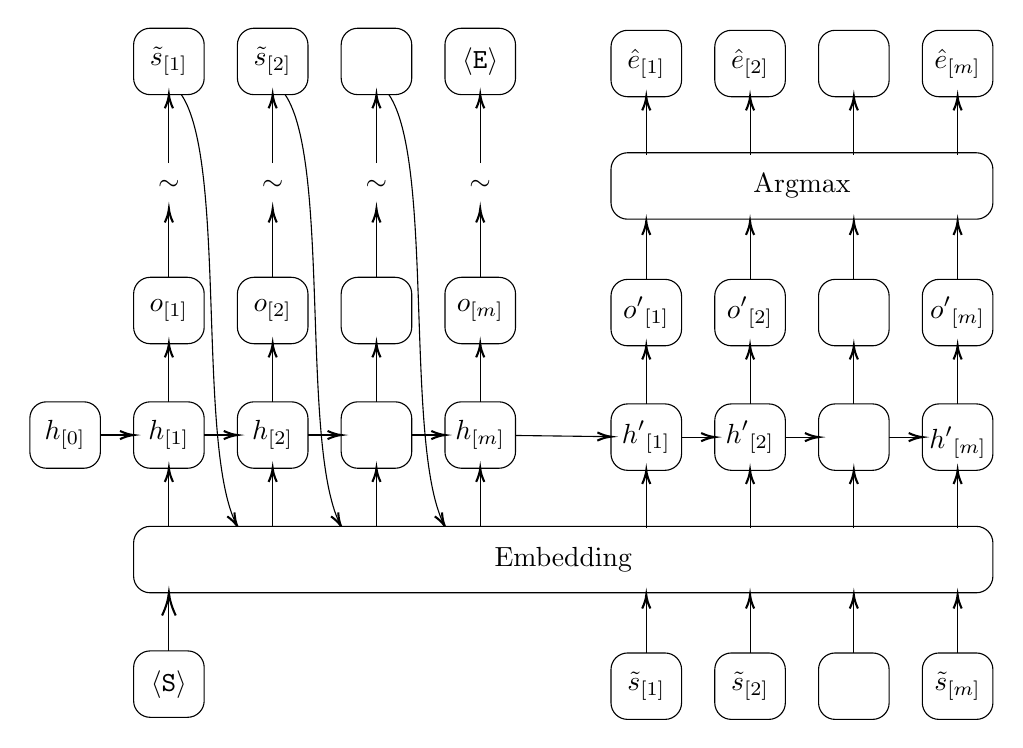
\begin{tikzpicture}[x=0.75pt,y=0.75pt,yscale=-1,xscale=1]
%uncomment if require: \path (0,355); %set diagram left start at 0, and has height of 355

%Curve Lines [id:da898021526375558]
\draw    (81,45) .. controls (102.77,77.16) and (88.54,212.5) .. (107.13,251.3) ;
\draw [shift={(108,253)}, rotate = 241.3] [color={rgb, 255:red, 0; green, 0; blue, 0 }  ][line width=0.75]    (6.56,-1.97) .. controls (4.17,-0.84) and (1.99,-0.18) .. (0,0) .. controls (1.99,0.18) and (4.17,0.84) .. (6.56,1.97)   ;
%Curve Lines [id:da8193603993553868]
\draw    (131,45) .. controls (152.77,77.16) and (138.54,212.5) .. (157.13,251.3) ;
\draw [shift={(158,253)}, rotate = 241.3] [color={rgb, 255:red, 0; green, 0; blue, 0 }  ][line width=0.75]    (6.56,-1.97) .. controls (4.17,-0.84) and (1.99,-0.18) .. (0,0) .. controls (1.99,0.18) and (4.17,0.84) .. (6.56,1.97)   ;
%Curve Lines [id:da9217609497584229]
\draw    (181,45) .. controls (202.77,77.16) and (188.54,212.5) .. (207.13,251.3) ;
\draw [shift={(208,253)}, rotate = 241.3] [color={rgb, 255:red, 0; green, 0; blue, 0 }  ][line width=0.75]    (6.56,-1.97) .. controls (4.17,-0.84) and (1.99,-0.18) .. (0,0) .. controls (1.99,0.18) and (4.17,0.84) .. (6.56,1.97)   ;

% Text Node
\draw  [fill={rgb, 255:red, 255; green, 255; blue, 255 }  ,fill opacity=1 ]  (58,261) .. controls (58,256.58) and (61.58,253) .. (66,253) -- (464,253) .. controls (468.42,253) and (472,256.58) .. (472,261) -- (472,277) .. controls (472,281.42) and (468.42,285) .. (464,285) -- (66,285) .. controls (61.58,285) and (58,281.42) .. (58,277) -- cycle  ;
\draw (265,269) node   [align=left] {\begin{minipage}[lt]{278.8pt}\setlength\topsep{0pt}
\begin{center}
Embedding
\end{center}

\end{minipage}};
% Text Node
\draw (75,269) node   [align=left] {\begin{minipage}[lt]{20.400000000000002pt}\setlength\topsep{0pt}
\begin{center}
\end{center}

\end{minipage}};
% Text Node
\draw (125,269) node   [align=left] {\begin{minipage}[lt]{20.400000000000002pt}\setlength\topsep{0pt}
\begin{center}
\end{center}

\end{minipage}};
% Text Node
\draw (175,269) node   [align=left] {\begin{minipage}[lt]{20.400000000000002pt}\setlength\topsep{0pt}
\begin{center}
\end{center}

\end{minipage}};
% Text Node
\draw (225,269) node   [align=left] {\begin{minipage}[lt]{20.400000000000002pt}\setlength\topsep{0pt}
\begin{center}
\end{center}

\end{minipage}};
% Text Node
\draw    (58,201) .. controls (58,196.58) and (61.58,193) .. (66,193) -- (84,193) .. controls (88.42,193) and (92,196.58) .. (92,201) -- (92,217) .. controls (92,221.42) and (88.42,225) .. (84,225) -- (66,225) .. controls (61.58,225) and (58,221.42) .. (58,217) -- cycle  ;
\draw (75,209) node   [align=left] {\begin{minipage}[lt]{20.400000000000002pt}\setlength\topsep{0pt}
\begin{center}
$\displaystyle \boldsymbol{h}_{[ 1]}$
\end{center}

\end{minipage}};
% Text Node
\draw    (108,201) .. controls (108,196.58) and (111.58,193) .. (116,193) -- (134,193) .. controls (138.42,193) and (142,196.58) .. (142,201) -- (142,217) .. controls (142,221.42) and (138.42,225) .. (134,225) -- (116,225) .. controls (111.58,225) and (108,221.42) .. (108,217) -- cycle  ;
\draw (125,209) node   [align=left] {\begin{minipage}[lt]{20.400000000000002pt}\setlength\topsep{0pt}
\begin{center}
$\displaystyle \boldsymbol{h}_{[ 2]}$
\end{center}

\end{minipage}};
% Text Node
\draw    (158,201) .. controls (158,196.58) and (161.58,193) .. (166,193) -- (184,193) .. controls (188.42,193) and (192,196.58) .. (192,201) -- (192,217) .. controls (192,221.42) and (188.42,225) .. (184,225) -- (166,225) .. controls (161.58,225) and (158,221.42) .. (158,217) -- cycle  ;
\draw (175,209) node   [align=left] {\begin{minipage}[lt]{20.400000000000002pt}\setlength\topsep{0pt}
\begin{center}
$\displaystyle \dotsc $
\end{center}

\end{minipage}};
% Text Node
\draw    (208,201) .. controls (208,196.58) and (211.58,193) .. (216,193) -- (234,193) .. controls (238.42,193) and (242,196.58) .. (242,201) -- (242,217) .. controls (242,221.42) and (238.42,225) .. (234,225) -- (216,225) .. controls (211.58,225) and (208,221.42) .. (208,217) -- cycle  ;
\draw (225,209) node   [align=left] {\begin{minipage}[lt]{20.400000000000002pt}\setlength\topsep{0pt}
\begin{center}
$\displaystyle \boldsymbol{h}_{[ m]}$
\end{center}

\end{minipage}};
% Text Node
\draw    (58,141) .. controls (58,136.58) and (61.58,133) .. (66,133) -- (84,133) .. controls (88.42,133) and (92,136.58) .. (92,141) -- (92,157) .. controls (92,161.42) and (88.42,165) .. (84,165) -- (66,165) .. controls (61.58,165) and (58,161.42) .. (58,157) -- cycle  ;
\draw (75,149) node   [align=left] {\begin{minipage}[lt]{20.400000000000002pt}\setlength\topsep{0pt}
\begin{center}
$\displaystyle \boldsymbol{o}_{[ 1]}$
\end{center}

\end{minipage}};
% Text Node
\draw    (108,141) .. controls (108,136.58) and (111.58,133) .. (116,133) -- (134,133) .. controls (138.42,133) and (142,136.58) .. (142,141) -- (142,157) .. controls (142,161.42) and (138.42,165) .. (134,165) -- (116,165) .. controls (111.58,165) and (108,161.42) .. (108,157) -- cycle  ;
\draw (125,149) node   [align=left] {\begin{minipage}[lt]{20.400000000000002pt}\setlength\topsep{0pt}
\begin{center}
$\displaystyle \boldsymbol{o}_{[ 2]}$
\end{center}

\end{minipage}};
% Text Node
\draw    (158,141) .. controls (158,136.58) and (161.58,133) .. (166,133) -- (184,133) .. controls (188.42,133) and (192,136.58) .. (192,141) -- (192,157) .. controls (192,161.42) and (188.42,165) .. (184,165) -- (166,165) .. controls (161.58,165) and (158,161.42) .. (158,157) -- cycle  ;
\draw (175,149) node   [align=left] {\begin{minipage}[lt]{20.400000000000002pt}\setlength\topsep{0pt}
\begin{center}
$\displaystyle \dotsc $
\end{center}

\end{minipage}};
% Text Node
\draw    (208,141) .. controls (208,136.58) and (211.58,133) .. (216,133) -- (234,133) .. controls (238.42,133) and (242,136.58) .. (242,141) -- (242,157) .. controls (242,161.42) and (238.42,165) .. (234,165) -- (216,165) .. controls (211.58,165) and (208,161.42) .. (208,157) -- cycle  ;
\draw (225,149) node   [align=left] {\begin{minipage}[lt]{20.400000000000002pt}\setlength\topsep{0pt}
\begin{center}
$\displaystyle \boldsymbol{o}_{[ m]}$
\end{center}

\end{minipage}};
% Text Node
\draw    (288,322) .. controls (288,317.58) and (291.58,314) .. (296,314) -- (314,314) .. controls (318.42,314) and (322,317.58) .. (322,322) -- (322,338) .. controls (322,342.42) and (318.42,346) .. (314,346) -- (296,346) .. controls (291.58,346) and (288,342.42) .. (288,338) -- cycle  ;
\draw (305,330) node   [align=left] {\begin{minipage}[lt]{20.400000000000002pt}\setlength\topsep{0pt}
\begin{center}
$\displaystyle \tilde{\boldsymbol{s}}_{[ 1]}$
\end{center}

\end{minipage}};
% Text Node
\draw (305,270) node   [align=left] {\begin{minipage}[lt]{20.400000000000002pt}\setlength\topsep{0pt}
\begin{center}
\end{center}

\end{minipage}};
% Text Node
\draw    (338,322) .. controls (338,317.58) and (341.58,314) .. (346,314) -- (364,314) .. controls (368.42,314) and (372,317.58) .. (372,322) -- (372,338) .. controls (372,342.42) and (368.42,346) .. (364,346) -- (346,346) .. controls (341.58,346) and (338,342.42) .. (338,338) -- cycle  ;
\draw (355,330) node   [align=left] {\begin{minipage}[lt]{20.400000000000002pt}\setlength\topsep{0pt}
\begin{center}
$\displaystyle \tilde{\boldsymbol{s}}_{[ 2]}$
\end{center}

\end{minipage}};
% Text Node
\draw    (388,322) .. controls (388,317.58) and (391.58,314) .. (396,314) -- (414,314) .. controls (418.42,314) and (422,317.58) .. (422,322) -- (422,338) .. controls (422,342.42) and (418.42,346) .. (414,346) -- (396,346) .. controls (391.58,346) and (388,342.42) .. (388,338) -- cycle  ;
\draw (405,330) node   [align=left] {\begin{minipage}[lt]{20.400000000000002pt}\setlength\topsep{0pt}
\begin{center}
$\displaystyle \dotsc $
\end{center}

\end{minipage}};
% Text Node
\draw    (438,322) .. controls (438,317.58) and (441.58,314) .. (446,314) -- (464,314) .. controls (468.42,314) and (472,317.58) .. (472,322) -- (472,338) .. controls (472,342.42) and (468.42,346) .. (464,346) -- (446,346) .. controls (441.58,346) and (438,342.42) .. (438,338) -- cycle  ;
\draw (455,330) node   [align=left] {\begin{minipage}[lt]{20.400000000000002pt}\setlength\topsep{0pt}
\begin{center}
$\displaystyle \tilde{\boldsymbol{s}}_{[ m]}$
\end{center}

\end{minipage}};
% Text Node
\draw (355,270) node   [align=left] {\begin{minipage}[lt]{20.400000000000002pt}\setlength\topsep{0pt}
\begin{center}
\end{center}

\end{minipage}};
% Text Node
\draw (405,270) node   [align=left] {\begin{minipage}[lt]{20.400000000000002pt}\setlength\topsep{0pt}
\begin{center}
\end{center}

\end{minipage}};
% Text Node
\draw (455,270) node   [align=left] {\begin{minipage}[lt]{20.400000000000002pt}\setlength\topsep{0pt}
\begin{center}
\end{center}

\end{minipage}};
% Text Node
\draw    (288,202) .. controls (288,197.58) and (291.58,194) .. (296,194) -- (314,194) .. controls (318.42,194) and (322,197.58) .. (322,202) -- (322,218) .. controls (322,222.42) and (318.42,226) .. (314,226) -- (296,226) .. controls (291.58,226) and (288,222.42) .. (288,218) -- cycle  ;
\draw (305,210) node   [align=left] {\begin{minipage}[lt]{20.400000000000002pt}\setlength\topsep{0pt}
\begin{center}
$\displaystyle \boldsymbol{h'}_{[ 1]}$
\end{center}

\end{minipage}};
% Text Node
\draw    (338,202) .. controls (338,197.58) and (341.58,194) .. (346,194) -- (364,194) .. controls (368.42,194) and (372,197.58) .. (372,202) -- (372,218) .. controls (372,222.42) and (368.42,226) .. (364,226) -- (346,226) .. controls (341.58,226) and (338,222.42) .. (338,218) -- cycle  ;
\draw (355,210) node   [align=left] {\begin{minipage}[lt]{20.400000000000002pt}\setlength\topsep{0pt}
\begin{center}
$\displaystyle \boldsymbol{h'}_{[ 2]}$
\end{center}

\end{minipage}};
% Text Node
\draw    (388,202) .. controls (388,197.58) and (391.58,194) .. (396,194) -- (414,194) .. controls (418.42,194) and (422,197.58) .. (422,202) -- (422,218) .. controls (422,222.42) and (418.42,226) .. (414,226) -- (396,226) .. controls (391.58,226) and (388,222.42) .. (388,218) -- cycle  ;
\draw (405,210) node   [align=left] {\begin{minipage}[lt]{20.400000000000002pt}\setlength\topsep{0pt}
\begin{center}
$\displaystyle \dotsc $
\end{center}

\end{minipage}};
% Text Node
\draw    (438,202) .. controls (438,197.58) and (441.58,194) .. (446,194) -- (464,194) .. controls (468.42,194) and (472,197.58) .. (472,202) -- (472,218) .. controls (472,222.42) and (468.42,226) .. (464,226) -- (446,226) .. controls (441.58,226) and (438,222.42) .. (438,218) -- cycle  ;
\draw (455,210) node   [align=left] {\begin{minipage}[lt]{20.400000000000002pt}\setlength\topsep{0pt}
\begin{center}
$\displaystyle \boldsymbol{h'}_{[ m]}$
\end{center}

\end{minipage}};
% Text Node
\draw    (288,142) .. controls (288,137.58) and (291.58,134) .. (296,134) -- (314,134) .. controls (318.42,134) and (322,137.58) .. (322,142) -- (322,158) .. controls (322,162.42) and (318.42,166) .. (314,166) -- (296,166) .. controls (291.58,166) and (288,162.42) .. (288,158) -- cycle  ;
\draw (305,150) node   [align=left] {\begin{minipage}[lt]{20.400000000000002pt}\setlength\topsep{0pt}
\begin{center}
$\displaystyle \boldsymbol{o'}_{[ 1]}$
\end{center}

\end{minipage}};
% Text Node
\draw    (338,142) .. controls (338,137.58) and (341.58,134) .. (346,134) -- (364,134) .. controls (368.42,134) and (372,137.58) .. (372,142) -- (372,158) .. controls (372,162.42) and (368.42,166) .. (364,166) -- (346,166) .. controls (341.58,166) and (338,162.42) .. (338,158) -- cycle  ;
\draw (355,150) node   [align=left] {\begin{minipage}[lt]{20.400000000000002pt}\setlength\topsep{0pt}
\begin{center}
$\displaystyle \boldsymbol{o'}_{[ 2]}$
\end{center}

\end{minipage}};
% Text Node
\draw    (388,142) .. controls (388,137.58) and (391.58,134) .. (396,134) -- (414,134) .. controls (418.42,134) and (422,137.58) .. (422,142) -- (422,158) .. controls (422,162.42) and (418.42,166) .. (414,166) -- (396,166) .. controls (391.58,166) and (388,162.42) .. (388,158) -- cycle  ;
\draw (405,150) node   [align=left] {\begin{minipage}[lt]{20.400000000000002pt}\setlength\topsep{0pt}
\begin{center}
$\displaystyle \dotsc $
\end{center}

\end{minipage}};
% Text Node
\draw    (438,142) .. controls (438,137.58) and (441.58,134) .. (446,134) -- (464,134) .. controls (468.42,134) and (472,137.58) .. (472,142) -- (472,158) .. controls (472,162.42) and (468.42,166) .. (464,166) -- (446,166) .. controls (441.58,166) and (438,162.42) .. (438,158) -- cycle  ;
\draw (455,150) node   [align=left] {\begin{minipage}[lt]{20.400000000000002pt}\setlength\topsep{0pt}
\begin{center}
$\displaystyle \boldsymbol{o'}_{[ m]}$
\end{center}

\end{minipage}};
% Text Node
\draw (75,89) node   [align=left] {\begin{minipage}[lt]{13.600000000000001pt}\setlength\topsep{0pt}
\begin{center}
$\displaystyle \sim $
\end{center}

\end{minipage}};
% Text Node
\draw (125,89) node   [align=left] {\begin{minipage}[lt]{13.600000000000001pt}\setlength\topsep{0pt}
\begin{center}
$\displaystyle \sim $
\end{center}

\end{minipage}};
% Text Node
\draw (175,89) node   [align=left] {\begin{minipage}[lt]{13.600000000000001pt}\setlength\topsep{0pt}
\begin{center}
$\displaystyle \sim $
\end{center}

\end{minipage}};
% Text Node
\draw (225,89) node   [align=left] {\begin{minipage}[lt]{13.600000000000001pt}\setlength\topsep{0pt}
\begin{center}
$\displaystyle \sim $
\end{center}

\end{minipage}};
% Text Node
\draw    (58,21) .. controls (58,16.58) and (61.58,13) .. (66,13) -- (84,13) .. controls (88.42,13) and (92,16.58) .. (92,21) -- (92,37) .. controls (92,41.42) and (88.42,45) .. (84,45) -- (66,45) .. controls (61.58,45) and (58,41.42) .. (58,37) -- cycle  ;
\draw (75,29) node   [align=left] {\begin{minipage}[lt]{20.400000000000002pt}\setlength\topsep{0pt}
\begin{center}
$\displaystyle \tilde{\boldsymbol{s}}_{[ 1]}$
\end{center}

\end{minipage}};
% Text Node
\draw    (108,21) .. controls (108,16.58) and (111.58,13) .. (116,13) -- (134,13) .. controls (138.42,13) and (142,16.58) .. (142,21) -- (142,37) .. controls (142,41.42) and (138.42,45) .. (134,45) -- (116,45) .. controls (111.58,45) and (108,41.42) .. (108,37) -- cycle  ;
\draw (125,29) node   [align=left] {\begin{minipage}[lt]{20.400000000000002pt}\setlength\topsep{0pt}
\begin{center}
$\displaystyle \tilde{\boldsymbol{s}}_{[ 2]}$
\end{center}

\end{minipage}};
% Text Node
\draw    (158,21) .. controls (158,16.58) and (161.58,13) .. (166,13) -- (184,13) .. controls (188.42,13) and (192,16.58) .. (192,21) -- (192,37) .. controls (192,41.42) and (188.42,45) .. (184,45) -- (166,45) .. controls (161.58,45) and (158,41.42) .. (158,37) -- cycle  ;
\draw (175,29) node   [align=left] {\begin{minipage}[lt]{20.400000000000002pt}\setlength\topsep{0pt}
\begin{center}
$\displaystyle \dotsc $
\end{center}

\end{minipage}};
% Text Node
\draw    (208,21) .. controls (208,16.58) and (211.58,13) .. (216,13) -- (234,13) .. controls (238.42,13) and (242,16.58) .. (242,21) -- (242,37) .. controls (242,41.42) and (238.42,45) .. (234,45) -- (216,45) .. controls (211.58,45) and (208,41.42) .. (208,37) -- cycle  ;
\draw (225,29) node   [align=left] {\begin{minipage}[lt]{20.400000000000002pt}\setlength\topsep{0pt}
\begin{center}
$\displaystyle \langle \mathtt{E} \rangle $
\end{center}

\end{minipage}};
% Text Node
\draw    (288,22) .. controls (288,17.58) and (291.58,14) .. (296,14) -- (314,14) .. controls (318.42,14) and (322,17.58) .. (322,22) -- (322,38) .. controls (322,42.42) and (318.42,46) .. (314,46) -- (296,46) .. controls (291.58,46) and (288,42.42) .. (288,38) -- cycle  ;
\draw (305,30) node   [align=left] {\begin{minipage}[lt]{20.400000000000002pt}\setlength\topsep{0pt}
\begin{center}
$\displaystyle \hat{\boldsymbol{e}}_{[ 1]}$
\end{center}

\end{minipage}};
% Text Node
\draw    (338,22) .. controls (338,17.58) and (341.58,14) .. (346,14) -- (364,14) .. controls (368.42,14) and (372,17.58) .. (372,22) -- (372,38) .. controls (372,42.42) and (368.42,46) .. (364,46) -- (346,46) .. controls (341.58,46) and (338,42.42) .. (338,38) -- cycle  ;
\draw (355,30) node   [align=left] {\begin{minipage}[lt]{20.400000000000002pt}\setlength\topsep{0pt}
\begin{center}
$\displaystyle \hat{\boldsymbol{e}}_{[ 2]}$
\end{center}

\end{minipage}};
% Text Node
\draw    (388,22) .. controls (388,17.58) and (391.58,14) .. (396,14) -- (414,14) .. controls (418.42,14) and (422,17.58) .. (422,22) -- (422,38) .. controls (422,42.42) and (418.42,46) .. (414,46) -- (396,46) .. controls (391.58,46) and (388,42.42) .. (388,38) -- cycle  ;
\draw (405,30) node   [align=left] {\begin{minipage}[lt]{20.400000000000002pt}\setlength\topsep{0pt}
\begin{center}
$\displaystyle \dotsc $
\end{center}

\end{minipage}};
% Text Node
\draw    (438,22) .. controls (438,17.58) and (441.58,14) .. (446,14) -- (464,14) .. controls (468.42,14) and (472,17.58) .. (472,22) -- (472,38) .. controls (472,42.42) and (468.42,46) .. (464,46) -- (446,46) .. controls (441.58,46) and (438,42.42) .. (438,38) -- cycle  ;
\draw (455,30) node   [align=left] {\begin{minipage}[lt]{20.400000000000002pt}\setlength\topsep{0pt}
\begin{center}
$\displaystyle \hat{\boldsymbol{e}}_{[ m]}$
\end{center}

\end{minipage}};
% Text Node
\draw    (8,201) .. controls (8,196.58) and (11.58,193) .. (16,193) -- (34,193) .. controls (38.42,193) and (42,196.58) .. (42,201) -- (42,217) .. controls (42,221.42) and (38.42,225) .. (34,225) -- (16,225) .. controls (11.58,225) and (8,221.42) .. (8,217) -- cycle  ;
\draw (25,209) node   [align=left] {\begin{minipage}[lt]{20.400000000000002pt}\setlength\topsep{0pt}
\begin{center}
$\displaystyle \boldsymbol{h}_{[ 0]}$
\end{center}

\end{minipage}};
% Text Node
\draw    (58,321) .. controls (58,316.58) and (61.58,313) .. (66,313) -- (84,313) .. controls (88.42,313) and (92,316.58) .. (92,321) -- (92,337) .. controls (92,341.42) and (88.42,345) .. (84,345) -- (66,345) .. controls (61.58,345) and (58,341.42) .. (58,337) -- cycle  ;
\draw (75,329) node   [align=left] {\begin{minipage}[lt]{20.400000000000002pt}\setlength\topsep{0pt}
\begin{center}
$\displaystyle \langle \mathtt{S} \rangle $
\end{center}

\end{minipage}};
% Text Node
\draw  [fill={rgb, 255:red, 255; green, 255; blue, 255 }  ,fill opacity=1 ]  (288,81) .. controls (288,76.58) and (291.58,73) .. (296,73) -- (464,73) .. controls (468.42,73) and (472,76.58) .. (472,81) -- (472,97) .. controls (472,101.42) and (468.42,105) .. (464,105) -- (296,105) .. controls (291.58,105) and (288,101.42) .. (288,97) -- cycle  ;
\draw (380,89) node   [align=left] {\begin{minipage}[lt]{122.4pt}\setlength\topsep{0pt}
\begin{center}
Argmax
\end{center}

\end{minipage}};
% Text Node
\draw (305,90) node   [align=left] {\begin{minipage}[lt]{20.400000000000002pt}\setlength\topsep{0pt}
\begin{center}
\end{center}

\end{minipage}};
% Text Node
\draw (355,90) node   [align=left] {\begin{minipage}[lt]{20.400000000000002pt}\setlength\topsep{0pt}
\begin{center}
\end{center}

\end{minipage}};
% Text Node
\draw (405,90) node   [align=left] {\begin{minipage}[lt]{20.400000000000002pt}\setlength\topsep{0pt}
\begin{center}
\end{center}

\end{minipage}};
% Text Node
\draw (455,90) node   [align=left] {\begin{minipage}[lt]{20.400000000000002pt}\setlength\topsep{0pt}
\begin{center}
\end{center}

\end{minipage}};
% Connection
\draw    (305,314) -- (305,288) ;
\draw [shift={(305,286)}, rotate = 450] [color={rgb, 255:red, 0; green, 0; blue, 0 }  ][line width=0.75]    (6.56,-1.97) .. controls (4.17,-0.84) and (1.99,-0.18) .. (0,0) .. controls (1.99,0.18) and (4.17,0.84) .. (6.56,1.97)   ;
% Connection
\draw    (355,314) -- (355,288) ;
\draw [shift={(355,286)}, rotate = 450] [color={rgb, 255:red, 0; green, 0; blue, 0 }  ][line width=0.75]    (6.56,-1.97) .. controls (4.17,-0.84) and (1.99,-0.18) .. (0,0) .. controls (1.99,0.18) and (4.17,0.84) .. (6.56,1.97)   ;
% Connection
\draw    (405,314) -- (405,288) ;
\draw [shift={(405,286)}, rotate = 450] [color={rgb, 255:red, 0; green, 0; blue, 0 }  ][line width=0.75]    (6.56,-1.97) .. controls (4.17,-0.84) and (1.99,-0.18) .. (0,0) .. controls (1.99,0.18) and (4.17,0.84) .. (6.56,1.97)   ;
% Connection
\draw    (455,314) -- (455,288) ;
\draw [shift={(455,286)}, rotate = 450] [color={rgb, 255:red, 0; green, 0; blue, 0 }  ][line width=0.75]    (6.56,-1.97) .. controls (4.17,-0.84) and (1.99,-0.18) .. (0,0) .. controls (1.99,0.18) and (4.17,0.84) .. (6.56,1.97)   ;
% Connection
\draw    (75,253) -- (75,227) ;
\draw [shift={(75,225)}, rotate = 450] [color={rgb, 255:red, 0; green, 0; blue, 0 }  ][line width=0.75]    (6.56,-1.97) .. controls (4.17,-0.84) and (1.99,-0.18) .. (0,0) .. controls (1.99,0.18) and (4.17,0.84) .. (6.56,1.97)   ;
% Connection
\draw    (125,253) -- (125,227) ;
\draw [shift={(125,225)}, rotate = 450] [color={rgb, 255:red, 0; green, 0; blue, 0 }  ][line width=0.75]    (6.56,-1.97) .. controls (4.17,-0.84) and (1.99,-0.18) .. (0,0) .. controls (1.99,0.18) and (4.17,0.84) .. (6.56,1.97)   ;
% Connection
\draw    (175,253) -- (175,227) ;
\draw [shift={(175,225)}, rotate = 450] [color={rgb, 255:red, 0; green, 0; blue, 0 }  ][line width=0.75]    (6.56,-1.97) .. controls (4.17,-0.84) and (1.99,-0.18) .. (0,0) .. controls (1.99,0.18) and (4.17,0.84) .. (6.56,1.97)   ;
% Connection
\draw    (225,253) -- (225,227) ;
\draw [shift={(225,225)}, rotate = 450] [color={rgb, 255:red, 0; green, 0; blue, 0 }  ][line width=0.75]    (6.56,-1.97) .. controls (4.17,-0.84) and (1.99,-0.18) .. (0,0) .. controls (1.99,0.18) and (4.17,0.84) .. (6.56,1.97)   ;
% Connection
\draw    (305,254) -- (305,228) ;
\draw [shift={(305,226)}, rotate = 450] [color={rgb, 255:red, 0; green, 0; blue, 0 }  ][line width=0.75]    (6.56,-1.97) .. controls (4.17,-0.84) and (1.99,-0.18) .. (0,0) .. controls (1.99,0.18) and (4.17,0.84) .. (6.56,1.97)   ;
% Connection
\draw    (355,254) -- (355,228) ;
\draw [shift={(355,226)}, rotate = 450] [color={rgb, 255:red, 0; green, 0; blue, 0 }  ][line width=0.75]    (6.56,-1.97) .. controls (4.17,-0.84) and (1.99,-0.18) .. (0,0) .. controls (1.99,0.18) and (4.17,0.84) .. (6.56,1.97)   ;
% Connection
\draw    (405,254) -- (405,228) ;
\draw [shift={(405,226)}, rotate = 450] [color={rgb, 255:red, 0; green, 0; blue, 0 }  ][line width=0.75]    (6.56,-1.97) .. controls (4.17,-0.84) and (1.99,-0.18) .. (0,0) .. controls (1.99,0.18) and (4.17,0.84) .. (6.56,1.97)   ;
% Connection
\draw    (455,254) -- (455,228) ;
\draw [shift={(455,226)}, rotate = 450] [color={rgb, 255:red, 0; green, 0; blue, 0 }  ][line width=0.75]    (6.56,-1.97) .. controls (4.17,-0.84) and (1.99,-0.18) .. (0,0) .. controls (1.99,0.18) and (4.17,0.84) .. (6.56,1.97)   ;
% Connection
\draw    (92,209) -- (106,209) ;
\draw [shift={(108,209)}, rotate = 180] [color={rgb, 255:red, 0; green, 0; blue, 0 }  ][line width=0.75]    (6.56,-1.97) .. controls (4.17,-0.84) and (1.99,-0.18) .. (0,0) .. controls (1.99,0.18) and (4.17,0.84) .. (6.56,1.97)   ;
% Connection
\draw    (142,209) -- (156,209) ;
\draw [shift={(158,209)}, rotate = 180] [color={rgb, 255:red, 0; green, 0; blue, 0 }  ][line width=0.75]    (6.56,-1.97) .. controls (4.17,-0.84) and (1.99,-0.18) .. (0,0) .. controls (1.99,0.18) and (4.17,0.84) .. (6.56,1.97)   ;
% Connection
\draw    (192,209) -- (206,209) ;
\draw [shift={(208,209)}, rotate = 180] [color={rgb, 255:red, 0; green, 0; blue, 0 }  ][line width=0.75]    (6.56,-1.97) .. controls (4.17,-0.84) and (1.99,-0.18) .. (0,0) .. controls (1.99,0.18) and (4.17,0.84) .. (6.56,1.97)   ;
% Connection
\draw    (242,209.21) -- (286,209.76) ;
\draw [shift={(288,209.79)}, rotate = 180.72] [color={rgb, 255:red, 0; green, 0; blue, 0 }  ][line width=0.75]    (6.56,-1.97) .. controls (4.17,-0.84) and (1.99,-0.18) .. (0,0) .. controls (1.99,0.18) and (4.17,0.84) .. (6.56,1.97)   ;
% Connection
\draw    (322,210) -- (336,210) ;
\draw [shift={(338,210)}, rotate = 180] [color={rgb, 255:red, 0; green, 0; blue, 0 }  ][line width=0.75]    (6.56,-1.97) .. controls (4.17,-0.84) and (1.99,-0.18) .. (0,0) .. controls (1.99,0.18) and (4.17,0.84) .. (6.56,1.97)   ;
% Connection
\draw    (372,210) -- (386,210) ;
\draw [shift={(388,210)}, rotate = 180] [color={rgb, 255:red, 0; green, 0; blue, 0 }  ][line width=0.75]    (6.56,-1.97) .. controls (4.17,-0.84) and (1.99,-0.18) .. (0,0) .. controls (1.99,0.18) and (4.17,0.84) .. (6.56,1.97)   ;
% Connection
\draw    (422,210) -- (436,210) ;
\draw [shift={(438,210)}, rotate = 180] [color={rgb, 255:red, 0; green, 0; blue, 0 }  ][line width=0.75]    (6.56,-1.97) .. controls (4.17,-0.84) and (1.99,-0.18) .. (0,0) .. controls (1.99,0.18) and (4.17,0.84) .. (6.56,1.97)   ;
% Connection
\draw    (75,193) -- (75,167) ;
\draw [shift={(75,165)}, rotate = 450] [color={rgb, 255:red, 0; green, 0; blue, 0 }  ][line width=0.75]    (6.56,-1.97) .. controls (4.17,-0.84) and (1.99,-0.18) .. (0,0) .. controls (1.99,0.18) and (4.17,0.84) .. (6.56,1.97)   ;
% Connection
\draw    (125,193) -- (125,167) ;
\draw [shift={(125,165)}, rotate = 450] [color={rgb, 255:red, 0; green, 0; blue, 0 }  ][line width=0.75]    (6.56,-1.97) .. controls (4.17,-0.84) and (1.99,-0.18) .. (0,0) .. controls (1.99,0.18) and (4.17,0.84) .. (6.56,1.97)   ;
% Connection
\draw    (175,193) -- (175,167) ;
\draw [shift={(175,165)}, rotate = 450] [color={rgb, 255:red, 0; green, 0; blue, 0 }  ][line width=0.75]    (6.56,-1.97) .. controls (4.17,-0.84) and (1.99,-0.18) .. (0,0) .. controls (1.99,0.18) and (4.17,0.84) .. (6.56,1.97)   ;
% Connection
\draw    (225,193) -- (225,167) ;
\draw [shift={(225,165)}, rotate = 450] [color={rgb, 255:red, 0; green, 0; blue, 0 }  ][line width=0.75]    (6.56,-1.97) .. controls (4.17,-0.84) and (1.99,-0.18) .. (0,0) .. controls (1.99,0.18) and (4.17,0.84) .. (6.56,1.97)   ;
% Connection
\draw    (305,194) -- (305,168) ;
\draw [shift={(305,166)}, rotate = 450] [color={rgb, 255:red, 0; green, 0; blue, 0 }  ][line width=0.75]    (6.56,-1.97) .. controls (4.17,-0.84) and (1.99,-0.18) .. (0,0) .. controls (1.99,0.18) and (4.17,0.84) .. (6.56,1.97)   ;
% Connection
\draw    (355,194) -- (355,168) ;
\draw [shift={(355,166)}, rotate = 450] [color={rgb, 255:red, 0; green, 0; blue, 0 }  ][line width=0.75]    (6.56,-1.97) .. controls (4.17,-0.84) and (1.99,-0.18) .. (0,0) .. controls (1.99,0.18) and (4.17,0.84) .. (6.56,1.97)   ;
% Connection
\draw    (405,194) -- (405,168) ;
\draw [shift={(405,166)}, rotate = 450] [color={rgb, 255:red, 0; green, 0; blue, 0 }  ][line width=0.75]    (6.56,-1.97) .. controls (4.17,-0.84) and (1.99,-0.18) .. (0,0) .. controls (1.99,0.18) and (4.17,0.84) .. (6.56,1.97)   ;
% Connection
\draw    (455,194) -- (455,168) ;
\draw [shift={(455,166)}, rotate = 450] [color={rgb, 255:red, 0; green, 0; blue, 0 }  ][line width=0.75]    (6.56,-1.97) .. controls (4.17,-0.84) and (1.99,-0.18) .. (0,0) .. controls (1.99,0.18) and (4.17,0.84) .. (6.56,1.97)   ;
% Connection
\draw    (75,133) -- (75,102) ;
\draw [shift={(75,100)}, rotate = 450] [color={rgb, 255:red, 0; green, 0; blue, 0 }  ][line width=0.75]    (6.56,-1.97) .. controls (4.17,-0.84) and (1.99,-0.18) .. (0,0) .. controls (1.99,0.18) and (4.17,0.84) .. (6.56,1.97)   ;
% Connection
\draw    (125,133) -- (125,102) ;
\draw [shift={(125,100)}, rotate = 450] [color={rgb, 255:red, 0; green, 0; blue, 0 }  ][line width=0.75]    (6.56,-1.97) .. controls (4.17,-0.84) and (1.99,-0.18) .. (0,0) .. controls (1.99,0.18) and (4.17,0.84) .. (6.56,1.97)   ;
% Connection
\draw    (175,133) -- (175,102) ;
\draw [shift={(175,100)}, rotate = 450] [color={rgb, 255:red, 0; green, 0; blue, 0 }  ][line width=0.75]    (6.56,-1.97) .. controls (4.17,-0.84) and (1.99,-0.18) .. (0,0) .. controls (1.99,0.18) and (4.17,0.84) .. (6.56,1.97)   ;
% Connection
\draw    (225,133) -- (225,102) ;
\draw [shift={(225,100)}, rotate = 450] [color={rgb, 255:red, 0; green, 0; blue, 0 }  ][line width=0.75]    (6.56,-1.97) .. controls (4.17,-0.84) and (1.99,-0.18) .. (0,0) .. controls (1.99,0.18) and (4.17,0.84) .. (6.56,1.97)   ;
% Connection
\draw    (42,209) -- (56,209) ;
\draw [shift={(58,209)}, rotate = 180] [color={rgb, 255:red, 0; green, 0; blue, 0 }  ][line width=0.75]    (6.56,-1.97) .. controls (4.17,-0.84) and (1.99,-0.18) .. (0,0) .. controls (1.99,0.18) and (4.17,0.84) .. (6.56,1.97)   ;
% Connection
\draw    (75,313) -- (75,287) ;
\draw [shift={(75,285)}, rotate = 450] [color={rgb, 255:red, 0; green, 0; blue, 0 }  ][line width=0.75]    (10.93,-3.29) .. controls (6.95,-1.4) and (3.31,-0.3) .. (0,0) .. controls (3.31,0.3) and (6.95,1.4) .. (10.93,3.29)   ;
% Connection
\draw    (75,78) -- (75,47) ;
\draw [shift={(75,45)}, rotate = 450] [color={rgb, 255:red, 0; green, 0; blue, 0 }  ][line width=0.75]    (6.56,-1.97) .. controls (4.17,-0.84) and (1.99,-0.18) .. (0,0) .. controls (1.99,0.18) and (4.17,0.84) .. (6.56,1.97)   ;
% Connection
\draw    (125,78) -- (125,47) ;
\draw [shift={(125,45)}, rotate = 450] [color={rgb, 255:red, 0; green, 0; blue, 0 }  ][line width=0.75]    (6.56,-1.97) .. controls (4.17,-0.84) and (1.99,-0.18) .. (0,0) .. controls (1.99,0.18) and (4.17,0.84) .. (6.56,1.97)   ;
% Connection
\draw    (175,78) -- (175,47) ;
\draw [shift={(175,45)}, rotate = 450] [color={rgb, 255:red, 0; green, 0; blue, 0 }  ][line width=0.75]    (6.56,-1.97) .. controls (4.17,-0.84) and (1.99,-0.18) .. (0,0) .. controls (1.99,0.18) and (4.17,0.84) .. (6.56,1.97)   ;
% Connection
\draw    (225,78) -- (225,47) ;
\draw [shift={(225,45)}, rotate = 450] [color={rgb, 255:red, 0; green, 0; blue, 0 }  ][line width=0.75]    (6.56,-1.97) .. controls (4.17,-0.84) and (1.99,-0.18) .. (0,0) .. controls (1.99,0.18) and (4.17,0.84) .. (6.56,1.97)   ;
% Connection
\draw    (305,134) -- (305,108) ;
\draw [shift={(305,106)}, rotate = 450] [color={rgb, 255:red, 0; green, 0; blue, 0 }  ][line width=0.75]    (6.56,-1.97) .. controls (4.17,-0.84) and (1.99,-0.18) .. (0,0) .. controls (1.99,0.18) and (4.17,0.84) .. (6.56,1.97)   ;
% Connection
\draw    (355,134) -- (355,108) ;
\draw [shift={(355,106)}, rotate = 450] [color={rgb, 255:red, 0; green, 0; blue, 0 }  ][line width=0.75]    (6.56,-1.97) .. controls (4.17,-0.84) and (1.99,-0.18) .. (0,0) .. controls (1.99,0.18) and (4.17,0.84) .. (6.56,1.97)   ;
% Connection
\draw    (405,134) -- (405,108) ;
\draw [shift={(405,106)}, rotate = 450] [color={rgb, 255:red, 0; green, 0; blue, 0 }  ][line width=0.75]    (6.56,-1.97) .. controls (4.17,-0.84) and (1.99,-0.18) .. (0,0) .. controls (1.99,0.18) and (4.17,0.84) .. (6.56,1.97)   ;
% Connection
\draw    (455,134) -- (455,108) ;
\draw [shift={(455,106)}, rotate = 450] [color={rgb, 255:red, 0; green, 0; blue, 0 }  ][line width=0.75]    (6.56,-1.97) .. controls (4.17,-0.84) and (1.99,-0.18) .. (0,0) .. controls (1.99,0.18) and (4.17,0.84) .. (6.56,1.97)   ;
% Connection
\draw    (305,74) -- (305,48) ;
\draw [shift={(305,46)}, rotate = 450] [color={rgb, 255:red, 0; green, 0; blue, 0 }  ][line width=0.75]    (6.56,-1.97) .. controls (4.17,-0.84) and (1.99,-0.18) .. (0,0) .. controls (1.99,0.18) and (4.17,0.84) .. (6.56,1.97)   ;
% Connection
\draw    (355,74) -- (355,48) ;
\draw [shift={(355,46)}, rotate = 450] [color={rgb, 255:red, 0; green, 0; blue, 0 }  ][line width=0.75]    (6.56,-1.97) .. controls (4.17,-0.84) and (1.99,-0.18) .. (0,0) .. controls (1.99,0.18) and (4.17,0.84) .. (6.56,1.97)   ;
% Connection
\draw    (405,74) -- (405,48) ;
\draw [shift={(405,46)}, rotate = 450] [color={rgb, 255:red, 0; green, 0; blue, 0 }  ][line width=0.75]    (6.56,-1.97) .. controls (4.17,-0.84) and (1.99,-0.18) .. (0,0) .. controls (1.99,0.18) and (4.17,0.84) .. (6.56,1.97)   ;
% Connection
\draw    (455,74) -- (455,48) ;
\draw [shift={(455,46)}, rotate = 450] [color={rgb, 255:red, 0; green, 0; blue, 0 }  ][line width=0.75]    (6.56,-1.97) .. controls (4.17,-0.84) and (1.99,-0.18) .. (0,0) .. controls (1.99,0.18) and (4.17,0.84) .. (6.56,1.97)   ;

\end{tikzpicture}}
    \caption{Graph generation. The output of the network are two sequences: one is a stochastic sequence $\Vector{\tilde{s}}$ representing the starting sequence of the graph. The other is a an ending sequence $\Vector{\hat{e}}$, predicted using $\Vector{\tilde{s}}$ as input. The two sequences are ultimately combined to produce the ordered edge sequence of a novel graph.}
    \label{fig:model-sampling}
\end{figure*}

\subsubsection*{Implementation details}\label{sec:implementation}
The model is implemented using the \texttt{PyTorch}\footnote{\url{https://github.com/marcopodda/grapher}} \cite{paszke2017pytorch} library; after an initial exploratory phase (not reported), some hyper-parameters (such as the number of recurrent layers) were fixed in advance. We use model selection with a 80\%-20\% splits to select the other hyper-parameters. We choose among 32 and 64 for the embedding dimension $d$, 128 and 256 for the recurrent state size $h$. We apply a dropout layer to the embedding layer, whose rate is chosen between 0.25 and 0.35. As recurrent cells, we use 2 layers of Gated Recurrent Units (GRU) \cite{cho2014gru}. As regards the learning parameters, we use the Adam \cite{kingma2015adam} optimizer with learning rate of 0.001, halved every 200 epochs. We train all models for a maximum of 2000 epochs, applying early stopping whenever the loss starts to plateau (we found a suitable empirical threshold after running a number of exploratory training instances).

\subsection{Experiments}
Following, we detail the experiments to assess our model, describing the datasets used for learning, the baselines we compared to, and the framework used for evaluation.

\subsubsection*{Datasets}\label{sec:datasets}
In our experiments, we evaluate our model on 3 synthetic datasets and 2 real-world datasets of molecular graphs. Every synthetic dataset represents graphs with particular node/edge dependencies. The rationale is to assess whether our approach is general enough to give good performances on very different graph distributions. Concretely, we use the following datasets:

\begin{itemize}
    \item LADDERS, a synthetic dataset of ladder graphs. We generate all possible ladder graphs having number of nodes $2n, n = 2, \ldots, 20$, and replicate them 10 times, resulting in a total size of 180 graphs. This dataset is inspired from the grids dataset used in \citep{you2018graphrnn}. In our case, we use ladder graphs because they have a similar node degree distribution, while being computationally manageable. In this dataset, the model has to capture very strong dependencies: the nodes of a ladder graph have degree of 3, except nodes at the four corners, which have degree of two. Any graph that does not respect this dependencies is not a ladder graph. An example of ladder graph is shown in Figure \ref{fig:ladder};
    \item COMMUNITY, a synthetic dataset of graphs with two-community structure. Community graphs are composed of two densely connected clusters of nodes, which are weakly connected between themselves. Here, the model has to capture the community structure. Community dependencies are very common in biological settings: for example, densely connected communities in metabolic networks often represent functional groups (see \eg \citep{girvan2002commstructsocialbionet}). To create this dataset, we firstly generate two clique graphs of random size between $8 \leq N \leq 20$. We then remove some edges randomly from the two clusters with probability $0.4$, and then connect the two communities with 1 or 2 edges at random. The generated dataset is composed of 1000 graphs. This dataset is similar to the COMMUNITY dataset used in \citep{you2018graphrnn}, which unfortunately we could not reproduce. An example of community graph is shown in Figure \ref{fig:community};
    \item EGO, a dataset of ego networks extracted from the Citeseer dataset \citep{giles1998citeseer}. In this case, the model has to capture the presence of a focal node (the \quotes{ego} node), which is connected to the majority of nodes in the graph, while the other nodes (the \quotes{alter} nodes) have weaker connectivity. This dependency is typical of social networks, and can be modeled with the BA model for preferential attachment. To create the dataset, we extract all possible ego networks of radius 2 from the Citeseer dataset. Thus, the path length between the ego node and the alter nodes is at most 2. The total number of graphs in the dataset is 1719. An example of ego graph is shown in Figure \ref{fig:ego};
    \item ENZYMES, a subset of 436 graphs taken from the ENZYMES dataset \citep{schomburg2004enzymes} (see Section \ref{sec:datasets} for details);
    \item PROTEINS, a subset of 794 graphs taken from the Dobson and Doig dataset \citep{dobson2003dd} (see Section \ref{sec:datasets} for details). In these two last datasets, the model should capture patterns of connectivity typical of molecules, such as functional groups or aromatic rings.
\end{itemize}
All datasets have a number of nodes comprised between 4 and 40, and a number of edges comprised between 2 and 130. Before training, we held out a portion of the dataset from testing purposes. In particular, for all datasets except LADDERS, we held out 30\% of graphs, and used them for evaluation. This held-out set acts as a random sample drawn from the corresponding unknown graph distribution.
\begin{figure*}[h!]
    \begin{subfigure}[b]{0.25\linewidth}
        \centering
        \resizebox{.55\textwidth}{!}{

\tikzset{every picture/.style={line width=0.75pt}} %set default line width to 0.75pt

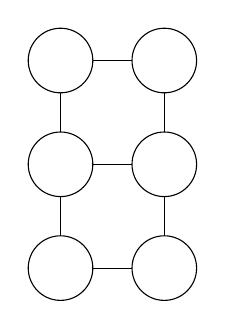
\begin{tikzpicture}[x=0.75pt,y=0.75pt,yscale=-1,xscale=1]
%uncomment if require: \path (0,166); %set diagram left start at 0, and has height of 166


% Text Node
\draw    (40, 30) circle [x radius= 15.56, y radius= 15.56]   ;
\draw (40,30) node   [align=left] {\begin{minipage}[lt]{13.600000000000001pt}\setlength\topsep{0pt}

\end{minipage}};
% Text Node
\draw    (90, 30) circle [x radius= 15.56, y radius= 15.56]   ;
\draw (90,30) node   [align=left] {\begin{minipage}[lt]{13.600000000000001pt}\setlength\topsep{0pt}

\end{minipage}};
% Text Node
\draw    (40, 80) circle [x radius= 15.56, y radius= 15.56]   ;
\draw (40,80) node   [align=left] {\begin{minipage}[lt]{13.600000000000001pt}\setlength\topsep{0pt}

\end{minipage}};
% Text Node
\draw    (90, 80) circle [x radius= 15.56, y radius= 15.56]   ;
\draw (90,80) node   [align=left] {\begin{minipage}[lt]{13.600000000000001pt}\setlength\topsep{0pt}

\end{minipage}};
% Text Node
\draw    (40, 130) circle [x radius= 15.56, y radius= 15.56]   ;
\draw (40,130) node   [align=left] {\begin{minipage}[lt]{13.600000000000001pt}\setlength\topsep{0pt}

\end{minipage}};
% Text Node
\draw    (90, 130) circle [x radius= 15.56, y radius= 15.56]   ;
\draw (90,130) node   [align=left] {\begin{minipage}[lt]{13.600000000000001pt}\setlength\topsep{0pt}

\end{minipage}};
% Connection
\draw    (55.56,30) -- (74.44,30) ;
% Connection
\draw    (40,45.56) -- (40,64.44) ;
% Connection
\draw    (90,45.56) -- (90,64.44) ;
% Connection
\draw    (40,95.56) -- (40,114.44) ;
% Connection
\draw    (90,95.56) -- (90,114.44) ;
% Connection
\draw    (55.56,130) -- (74.44,130) ;
% Connection
\draw    (55.56,80) -- (74.44,80) ;

\end{tikzpicture}}
        \caption{Ladder graph.}
        \label{fig:ladder}
    \end{subfigure}
    \begin{subfigure}[b]{0.43\linewidth}
        \centering
        \resizebox{.8\textwidth}{!}{

\tikzset{every picture/.style={line width=0.75pt}} %set default line width to 0.75pt

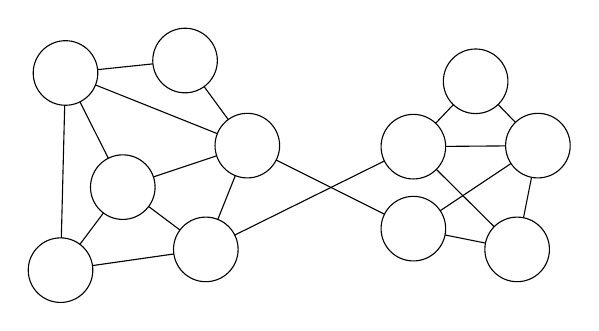
\begin{tikzpicture}[x=0.75pt,y=0.75pt,yscale=-1,xscale=1]
%uncomment if require: \path (0,158); %set diagram left start at 0, and has height of 158


% Text Node
\draw    (32.4, 26) circle [x radius= 15.56, y radius= 15.56]   ;
\draw (32.4,26) node   [align=left] {\begin{minipage}[lt]{13.600000000000001pt}\setlength\topsep{0pt}

\end{minipage}};
% Text Node
\draw    (90, 20) circle [x radius= 15.56, y radius= 15.56]   ;
\draw (90,20) node   [align=left] {\begin{minipage}[lt]{13.600000000000001pt}\setlength\topsep{0pt}

\end{minipage}};
% Text Node
\draw    (60, 81) circle [x radius= 15.56, y radius= 15.56]   ;
\draw (60,81) node   [align=left] {\begin{minipage}[lt]{13.600000000000001pt}\setlength\topsep{0pt}

\end{minipage}};
% Text Node
\draw    (120, 61) circle [x radius= 15.56, y radius= 15.56]   ;
\draw (120,61) node   [align=left] {\begin{minipage}[lt]{13.600000000000001pt}\setlength\topsep{0pt}

\end{minipage}};
% Text Node
\draw    (30, 121) circle [x radius= 15.56, y radius= 15.56]   ;
\draw (30,121) node   [align=left] {\begin{minipage}[lt]{13.600000000000001pt}\setlength\topsep{0pt}

\end{minipage}};
% Text Node
\draw    (100, 111) circle [x radius= 15.56, y radius= 15.56]   ;
\draw (100,111) node   [align=left] {\begin{minipage}[lt]{13.600000000000001pt}\setlength\topsep{0pt}

\end{minipage}};
% Text Node
\draw    (230, 30) circle [x radius= 15.56, y radius= 15.56]   ;
\draw (230,30) node   [align=left] {\begin{minipage}[lt]{13.600000000000001pt}\setlength\topsep{0pt}

\end{minipage}};
% Text Node
\draw    (200, 61.5) circle [x radius= 15.56, y radius= 15.56]   ;
\draw (200,61.5) node   [align=left] {\begin{minipage}[lt]{13.600000000000001pt}\setlength\topsep{0pt}

\end{minipage}};
% Text Node
\draw    (260, 61) circle [x radius= 15.56, y radius= 15.56]   ;
\draw (260,61) node   [align=left] {\begin{minipage}[lt]{13.600000000000001pt}\setlength\topsep{0pt}

\end{minipage}};
% Text Node
\draw    (200, 101) circle [x radius= 15.56, y radius= 15.56]   ;
\draw (200,101) node   [align=left] {\begin{minipage}[lt]{13.600000000000001pt}\setlength\topsep{0pt}

\end{minipage}};
% Text Node
\draw    (250, 111) circle [x radius= 15.56, y radius= 15.56]   ;
\draw (250,111) node   [align=left] {\begin{minipage}[lt]{13.600000000000001pt}\setlength\topsep{0pt}

\end{minipage}};
% Connection
\draw    (219.27,41.26) -- (210.73,50.24) ;
% Connection
\draw    (240.82,41.18) -- (249.18,49.82) ;
% Connection
\draw    (211.06,72.44) -- (238.94,100.06) ;
% Connection
\draw    (247.05,69.63) -- (212.95,92.37) ;
% Connection
\draw    (215.26,104.05) -- (234.74,107.95) ;
% Connection
\draw    (253.05,95.74) -- (256.95,76.26) ;
% Connection
\draw    (186.06,68.4) -- (113.94,104.1) ;
% Connection
\draw    (114.22,75.45) -- (105.78,96.55) ;
% Connection
\draw    (110.81,48.44) -- (99.19,32.56) ;
% Connection
\draw    (105.55,55.23) -- (46.85,31.77) ;
% Connection
\draw    (32.01,41.55) -- (30.39,105.45) ;
% Connection
\draw    (39.38,39.91) -- (53.02,67.09) ;
% Connection
\draw    (47.87,24.39) -- (74.53,21.61) ;
% Connection
\draw    (50.67,93.45) -- (39.33,108.55) ;
% Connection
\draw    (45.4,118.8) -- (84.6,113.2) ;
% Connection
\draw    (72.45,90.33) -- (87.55,101.67) ;
% Connection
\draw    (74.76,76.08) -- (105.24,65.92) ;
% Connection
\draw    (186.08,94.04) -- (133.92,67.96) ;
% Connection
\draw    (215.56,61.37) -- (244.44,61.13) ;

\end{tikzpicture}}
        \caption{Community graph.}
        \label{fig:community}
    \end{subfigure}
    \begin{subfigure}[b]{0.30\linewidth}
        \centering
        \resizebox{.8\textwidth}{!}{

\tikzset{every picture/.style={line width=0.75pt}} %set default line width to 0.75pt

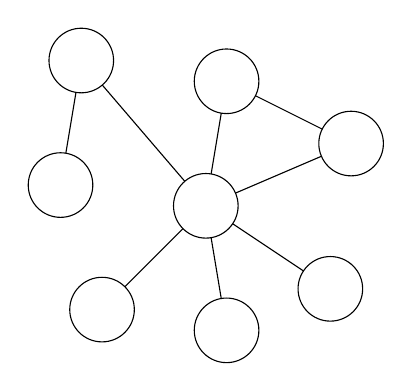
\begin{tikzpicture}[x=0.75pt,y=0.75pt,yscale=-1,xscale=1]
%uncomment if require: \path (0,194); %set diagram left start at 0, and has height of 194


% Text Node
\draw    (40, 30) circle [x radius= 15.56, y radius= 15.56]   ;
\draw (40,30) node   [align=left] {\begin{minipage}[lt]{13.600000000000001pt}\setlength\topsep{0pt}

\end{minipage}};
% Text Node
\draw    (100, 100) circle [x radius= 15.56, y radius= 15.56]   ;
\draw (100,100) node   [align=left] {\begin{minipage}[lt]{13.600000000000001pt}\setlength\topsep{0pt}

\end{minipage}};
% Text Node
\draw    (110, 40) circle [x radius= 15.56, y radius= 15.56]   ;
\draw (110,40) node   [align=left] {\begin{minipage}[lt]{13.600000000000001pt}\setlength\topsep{0pt}

\end{minipage}};
% Text Node
\draw    (170, 70) circle [x radius= 15.56, y radius= 15.56]   ;
\draw (170,70) node   [align=left] {\begin{minipage}[lt]{13.600000000000001pt}\setlength\topsep{0pt}

\end{minipage}};
% Text Node
\draw    (160, 140) circle [x radius= 15.56, y radius= 15.56]   ;
\draw (160,140) node   [align=left] {\begin{minipage}[lt]{13.600000000000001pt}\setlength\topsep{0pt}

\end{minipage}};
% Text Node
\draw    (110, 160) circle [x radius= 15.56, y radius= 15.56]   ;
\draw (110,160) node   [align=left] {\begin{minipage}[lt]{13.600000000000001pt}\setlength\topsep{0pt}

\end{minipage}};
% Text Node
\draw    (50, 150) circle [x radius= 15.56, y radius= 15.56]   ;
\draw (50,150) node   [align=left] {\begin{minipage}[lt]{13.600000000000001pt}\setlength\topsep{0pt}

\end{minipage}};
% Text Node
\draw    (30, 90) circle [x radius= 15.56, y radius= 15.56]   ;
\draw (30,90) node   [align=left] {\begin{minipage}[lt]{13.600000000000001pt}\setlength\topsep{0pt}

\end{minipage}};
% Connection
\draw    (89.88,88.19) -- (50.12,41.81) ;
% Connection
\draw    (89,111) -- (61,139) ;
% Connection
\draw    (102.56,115.35) -- (107.44,144.65) ;
% Connection
\draw    (112.95,108.63) -- (147.05,131.37) ;
% Connection
\draw    (114.3,93.87) -- (155.7,76.13) ;
% Connection
\draw    (102.56,84.65) -- (107.44,55.35) ;
% Connection
\draw    (123.92,46.96) -- (156.08,63.04) ;
% Connection
\draw    (37.44,45.35) -- (32.56,74.65) ;

\end{tikzpicture}}
        \caption{Ego graph.}
        \label{fig:ego}
    \end{subfigure}
    \caption{Three examples of synthetic graphs from the datasets used during the evaluation.}
    \label{fig:synthetic-graphs}
\end{figure*}
For the LADDERS dataset, we held out 10\% of graphs in a stratified fashion. In practice, the held-out set for LADDERS is composed of the same 18 unique ladder graphs found in the training set. To motivate this choice, let us clarify the role of the LADDERS dataset: its purpose is not to evaluate generalization capability, but to show that adaptive models can overfit hard node/edge dependencies among nodes, while non-adaptive models (such as the ER and BA models) cannot. The statistics of the datasets used for evaluation are presented in Table \ref{tab:generation-datasets}.

\begin{table}[h!]
    \footnotesize
    \centering
    \caption{Statistics of datasets used in the experiments.}
    \label{tab:generation-datasets}
    \renewcommand{\arraystretch}{1.2}
    \begin{tabular}{lcccc}
        \toprule
         \textbf{Dataset} & \textbf{No. of graphs} & \textbf{Test size} & \textbf{Avg. no. of nodes} & \textbf{Avg. no. of edges}\\
         \midrule
         LADDERS & 180 & 18 & 21.00 & 29.50 \\
         COMMUNITY & 1000 & 300 & 24.38 & 88.58 \\
         EGO & 1719 & 516 & 13.02 & 18.51 \\
         TREES & 780 & 180 & 109.14 & 108.14 \\
         ENZYMES & 436 & 130 & 26.14 & 51.16 \\
         PROTEINS & 794 & 238 & 20.49 & 38.67 \\
        \bottomrule
    \end{tabular}
\end{table}

\subsubsection*{Baselines}
We compare against four baseline models. Two of them are classical generative models of graphs coming from graph theory literature, namely the ER and BA models. The rationale behind this choice is to assess whether our model is able to perform better than random models that model graph connectivity independently (ER), or consider just one simple edge dependency (BA, where the probability of an edge is a function of the node degree).

The ER model has two parameters: $n$, the number of nodes of the graph to be generated, and $P$, the probability of adding an edge between a pair of nodes. The generative process of the ER model can be described informally as follows: first, pick $n$, then, for each possible pair of nodes, sample a Bernoulli random variable with probability $P$, and connect the two nodes according to the sampled value. We sample $n$ from the empirical distribution of the number of nodes in the datasets, and choose $P$ from a grid of values. The best value of $P$ is obtained by minimizing the earth mover distance between the empirical distributionand the generated distribution of graph properties

Similarly, the BA model has two parameters: $n$, the number of nodes of the graph to be generated, and $M$, a maximum number of nodes a node can be connected to. The generative process for a BA graph proceeds incrementally: given an already formed graph, add a new node and connect it (or not) to at most $M$ nodes with probability proportional to the nodes degree. In our experiments, the two parameters of the BA model are optimized in a similar fashion as the ER model.

Besides graph theory baslines, we also compare to a strong Deep-Learning based generative baseline. In particular, we choose the GraphRNN model of \citet{you2018graphrnn}, which holds state-of-the-art performances in the graph generation task. We implemented the model according to the original code repository provided by the authors, following their implementation and their hyper-parameters configuration closely.

Lastly, we introduce a third baseline model, a recurrent neural network with GRU cells that is trained to predict the adjacency matrix of the graph one entry at a time. We call this baseline GRU-B(aseline) from now on. It is arguably the simplest model one can come up with to model graph generation in a recurrent fashion, with the limitation that it has to sample $n(n-1)/2$ entries to fully specify the adjacency matrix of an undirected graph with $n$ nodes, making it susceptible to learning issues induced by long-term dependencies \citep{bengio1994learninglongtermdependenciesdifficult}. Clearly, even though Deep-Learning based, this baseline has purposedly limited expressiveness with respect of our model and GraphRNN.

\subsubsection*{Evaluation Framework}
We assess our model against the baselines following the quantitative and qualitative evaluation principles described in Section \ref{sec:evaluation-generative-graphs}. The experiments are described as follows:
\begin{itemize}
    \item our first experiment consists in evaluating the model quantitatively. To be sure to detect overfitting, we generate large samples. Specifically, we generate two samples of size 1000 and 5000 from all the candidates. For each of sample, we measure the novelty and uniqueness of the generated graphs. Despite using chemical datasets (ENZYMES and PROTEINS), we do not evaluate chemical validity because we are concerned about generating unlabeled graphs; thus, chemical validity cannot be assessed in our case. Finally, we also measure the time that each model takes to generate the 5000 graph sample;
    \item the second experiment is of qualitative nature. In practice, we assess how much the generated samples resemble a random sample from the graph distribution of reference. To do so, we first generate from all the models a sample of equal size to the held-out test set. Then, on each sample, we evaluate the \gls{kld} on a set of graph statistics, collected in the generated sample and in the test sample. Specifically, we evaluate Average Degree Distribution (ADD), Average Clustering Coefficient (ACC), and Average Orbit Count (AOC). Note that, since each graph can have a different number of nodes, the vectors of statistics for each graph have different lengths in general. Therefore, for each of the two samples, we concatenate the graph statistics vectors into a unique vector, on which we fit an histogram of 100 bins. The \gls{kld} is calculated on the two resulting histograms. This process is repeated 10 times, each time drawing a novel sample from the models.
\end{itemize}
Lastly, we provide a study on how using different node orderings affects performances. To do so, we compare our proposed model with variants where graphs are preprocessed used different node orderings. The five analyzed variants are:
\begin{itemize}
    \item \emph{Random}: the node ordering is a random permutation of the nodes. This strategy is expected to perform very poorly, since the model does not see consistent connectivity patterns during training;
    \item \emph{BF Random}: the node ordering strategy proposed by \citet{you2018graphrnn}. Such strategy is very similar to ours (in fact, our strategy is inspired by it), but differs in that, each time a graph is picked from the training set at different epochs, the root node for the visit can be different. In principle, this means that the model is trained on every possible node permutation induced by a breadth-first (BF) visit of the graph. On one hand, this strategy acts as a regularizer, since at each epoch the training set changes completely. On the other hand, however, changing the node ordering at each epoch could in principle prevent our model from focusing on useful connectivity patterns, simply because they are "masked" away by different node permutations;
    \item \emph{DF Random}: the same strategy as BF random, but using depth-first (DF) visit instead;
    \item \emph{DF}: a variant of our proposed strategy which uses depth-first traversal instead of breadth-first;
    \item \emph{SMILES}: the node ordering imposed by the SMILES encoding of the graph. This strategy is available only in the PROTEINS and ENZYMES datasets, which consist of molecular graphs;
\end{itemize}
Our first experiment for this analysis consists in training the models with the alternative node ordering strategies for a large number of epochs without regularization. In practice, we try to overfit the dataset on purpose. The idea is to assess whether the alternative node ordering strategies are able to memorize connectivity patterns (hence, given proper regularization, are able to generalize to unseen ones). In our second experiment, we perform a qualitative analysis comparing the performances of our model to the different variants.

\subsection{Results}
Here, we present the results of our experiments. We divide the analysis of the results into a quantitative and qualitative sections for readability purposes.

\subsubsection*{Quantitative Analysis}
Table \ref{tab:graph-quantitative} shows the results of our quantitative experiments. The best performances in terms of novelty and uniqueness are obtained consistently by the ER and BA models; this was expected, since by definition they produce random graphs, hence very likely to be different from the training set, as well as from the generated sample. One exception is the EGO dataset, where random models score poorly with respect to the competitors. We argue that this result is due to the nature of the EGO dataset, which is composed of graphs with very weak connectivity (except for the ego nodes) and a very low number of cycles. With such characteristics, it is easier for a random model to produce duplicates or overfit the training sample, just by setting the parameters that regulate connectivity to small values.
\begin{table}[h!]
    \footnotesize
    \centering
    \caption{Results of the quantitative analysis of the generated samples. In the leftmost column, both the metric of interest as well as the sample size (either 1000 or 5000) is specified. Best performances of models based on RNNs are bolded.}
    \label{tab:graph-quantitative}
    \renewcommand{\arraystretch}{1.2}
    \begin{tabular}{lcccccccc}
        \toprule
         \textbf{Dataset} & \textbf{Metric} & \textbf{ER} & \textbf{BA} & \textbf{GRU-B} & \textbf{GraphRNN} & \textbf{Ours} \\
         \midrule
          & Novelty@1000              & $\mathbf{1.00}$ & $\mathbf{1.00}$ & $0.81$          & $0.99$          & $\mathbf{1.00}$\\
          & Novelty@5000              & $\mathbf{1.00}$ & $\mathbf{1.00}$ & $0.83$          & $\mathbf{1.00}$          & $\mathbf{1.00}$\\
          LADDERS & Uniqueness@1000   & $0.93$ & $0.68$ & $0.06$          & $\mathbf{0.54}$ & $0.27$\\
          & Uniqueness@5000           & $0.89$ & $0.51$ & $0.03$          & $\mathbf{0.41}$ & $0.23$\\
          & Time@5000                 & $<$1s    & 1s       & 6m32s             & 17m06s            & 3m38s\\
         \midrule
          & Novelty@1000              & $\mathbf{1.00}$ & $\mathbf{1.00}$ & $\mathbf{1.00}$ & $\mathbf{1.00}$ & $\mathbf{1.00}$\\
          & Novelty@5000              & $\mathbf{1.00}$ & $\mathbf{1.00}$ & $\mathbf{1.00}$ & $\mathbf{1.00}$ & $\mathbf{1.00}$\\
          COMMUNITY & Uniqueness@1000 & $\mathbf{1.00}$ & $\mathbf{1.00}$ & $\mathbf{1.00}$ & $\mathbf{1.00}$ & $\mathbf{1.00}$\\
          & Uniqueness@5000           & $\mathbf{1.00}$ & $\mathbf{1.00}$ & $\mathbf{1.00}$ & $\mathbf{1.000}$ & $\mathbf{1.00}$\\
          & Time@5000                 & 3s       & 5s       & 7m25s             & 52m26s            & 8m58s\\
         \midrule
          & Novelty@1000              & $0.81$ & $0.85$ & $0.74$          & $\mathbf{1.00}$ & $0.96$\\
          & Novelty@5000              & $0.85$ & $0.81$ & $0.72$          & $\mathbf{1.00}$ & $0.96$\\
          EGO & Uniqueness@1000       & $0.65$ & $0.76$ & $0.61$          & $\mathbf{1.00}$ & $0.95$\\
          & Uniqueness@5000           & $0.53$ & $0.65$ & $0.47$          & $\mathbf{1.00}$ & $0.90$\\
          & Time@5000                 & 1s       & 1s       & 6m01s             & 1h10m16s          & 3m23s\\
         \midrule
          & Novelty@1000              & $\mathbf{1.00}$ & $\mathbf{1.00}$ & $\mathbf{1.00}$          & $0.97$          & $\mathbf{1.00}$\\
          & Novelty@5000              & $\mathbf{1.00}$ & $\mathbf{1.00}$ & $\mathbf{1.00}$          & $0.98$          & $\mathbf{1.00}$\\
          ENZYMES & Uniqueness@1000   & $0.99$ & $0.98$ & $0.77$          & $\mathbf{0.99}$ & $0.98$\\
          & Uniqueness@5000           & $\mathbf{1.00}$ & $0.97$ & $0.54$          & $\mathbf{0.97}$ & $\mathbf{0.97}$\\
          & Time@5000                 & 3s       & 3s       & 7m19s             & 52m24s            & 4m41s\\
        \midrule
          & Novelty@1000              & $0.99$ & $\mathbf{1.00}$ & $0.91$          & $0.86$          & $\mathbf{0.91}$\\
          & Novelty@5000              & $\mathbf{1.00}$ & $\mathbf{1.00}$ & $0.91$          & $0.87$          & $\mathbf{0.93}$\\
          PROTEIN & Uniqueness@1000  & $0.97$ & $0.91$ & $0.74$          & $0.90$          & $\mathbf{0.93}$\\
          & Uniqueness@5000           & $0.95$ & $0.89$ & $0.47$          & $0.83$          & $\mathbf{0.88}$\\
          & Time@5000                 & $<$1s    & 4s       & 6m29s             & 54m07s            & 3m44s\\
          \bottomrule
    \end{tabular}
\end{table}
In contrast, our model and GraphRNN consistently generate graphs with high novelty and uniqueness rates in almost all scenarios. The only exception to this trend is the ladders dataset, where both our model and GraphRNN overfit (they tend to generate the same graphs over and over), while random models do not. However, we remark the peculiarity of the LADDERS we mentioned in Section \ref{sec:datasets}. The main purpose of that particular dataset is to show that random models are unable to learn the strong edge dependency of ladder graphs. Thus, the analysis of novelty and uniqueness must be put into perspective by the qualitative analysis, to see whether structural dependencies have also been learned.

The GRU-B model greatly under-performs in all but the COMMUNITY dataset. From this result alone, one could legitimately infer that the model is not generalizing to unseen adjacency matrices. However, the qualitative analysis and the high value of the training loss (not shown) suggest that the model cannot perform any better. This provides evidence that a simple recurrent model such as GRU-B, at least in this form, is not well suited for the task of graph generation.

Our model obtainx excellent novelty and uniqueness scores in every dataset except LADDERS (for reasons explained above), with the notable mention of the PROTEINS dataset, where it obtains the best performances in every scored metric with a margin of 0.02 to 0.06 points with respect to the GraphRNN model. On the other hand, the GraphRNN model obtains a perfect score in the EGO dataset, beating our model with a margin of 0.3 to 0.1 points. However, our model is the most consistent across all the datsets, obtaining a score of above 0.87 in all considered scores in every dataset except LADDERS.

Note how all models obtain a perfect score in the COMMUNITY dataset. This can be explained by considering the nature of the COMMUNITY dataset, whose graphs are essentially composed by two random graphs weakly connected among each other. Thus, since generating a graph from that distribution is very similar to generating one at random, samples are highly likely to be different from each other.

As regards sampling time, random models are the fastest during generation; this was expected, since they have only 2 parameters, while all RNN-based models have a larger number of parameters. Among the RNN-based models, our model is the fastest at generating new samples. One exception is the COMMUNITY dataset, where however it elapses only 1.5 minutes more than the winning model, GRU-B. In contrast, the GraphRNN model has sampling times 5 to 20 times slower than our model. For completeness, however, we report that while we sampled from the GraphRNN model with batch size of 1 to achieve a fair comparison, its implementation allows to draw samples in batches, greatly speeding up the sampling process.

Table \ref{tab:graph-quantitative-rank} shows the mean rank of the models for each considered metric (except time), averaged over all datasets. More precisely, for a given metric, we collect the scores of all models on that particular metric, sort the corresponding vector in descending order from highest to lowest score. The order of the vector is the corresponding rank. The ranks are finally averaged across all datasets, to provide a measure of how models behave globally. Results show that the BA model has the highest mean rank as regards novelty on a sample size of 1000 (for the reasons discussed above), while GraphRNN has the highest mean rank as regards novelty on a sample of 5000. Our model obtains the highest mean rank on uniqueness, on both sample sizes.
\begin{table}[h!]
    \footnotesize
    \centering
    \caption{Mean ranks on all considered quantitative metrics except time, obtained by the examined models over all datasets. Best performances of models based on RNNs are bolded.}
    \label{tab:graph-quantitative-rank}
    \renewcommand{\arraystretch}{1.2}
    \begin{tabular}{cccccccc}
          \toprule
          \textbf{Metric} & \textbf{ER} & \textbf{BA} & \textbf{GRU-B} & \textbf{GraphRNN} & \textbf{Ours} \\
          \midrule
          Novelty@1000    & $3.00$ & $2.60$ & $3.20$ & $3.20$          & $\textbf{3.00}$\\
          Novelty@5000    & $3.00$ & $2.60$          & $4.00$ & $\textbf{2.40}$ & $3.00$\\
          Uniqueness@1000 & $2.60$ & $3.40$          & $3.20$ & $3.40$          & $\textbf{2.40}$\\
          Uniqueness@5000 & $2.60$ & $4.00$          & $3.40$ & $2.80$          & $\textbf{2.20}$\\
          \bottomrule
    \end{tabular}
\end{table}

\subsubsection*{Qualitative Analysis}
Table \ref{tab:graph-qualitative} shows the results of the qualitative evaluation of the models. We remark that lower values are better.
It can be clearly seen how random models are unable to learn complex dependencies, scoring poorly on all datasets in every considered metric. One exception is the EGO dataset, where both the ER and BA models obtain the best KLD for the AOC metric (orbit counts) with 0.07 and 0.09, respectively (results are indistinguishable since the standard deviation intervals overlap). This result is in accordance with the argument made in the quantitative analysis, where we explained that random models fit the EGO with a small connectivity parameter. Since ego graphs have very low higher-order connectivity, in this case they are able to capture the correct orbit counts distribution. In the LADDERS dataset, the BA model obtains the best ACC (clustering coefficient), scoring $0$ in all experiments. A similar argument can be made in this case: in fact, the clustering coefficient of ladder graphs is 0 by construction. Thus, it can be easily emulated with a very small connectivity parameter value. In contrast, note how the BA model completely fails at generating graphs with the correct node degree distribution, scoring the worst among all datasets. A similar trend happens to the ER model, providing evidence that random models are suited to model only a small subset of graph distributions.
\begin{table}[h!]
    \scriptsize
    \caption{Results of the qualitative analysis of the generated samples. The three metrics considered are KLDs calculated on Average Degree Distribution (ADD), Average Clustering Coefficient (ACC), and Average Orbit Count (AOD). Best performances are bolded.}
    \label{tab:graph-qualitative}
    \renewcommand{\arraystretch}{1.2}
    \makebox[\textwidth]{
    \begin{tabular}{lcccccc}
        \toprule
         \textbf{Dataset} & \textbf{Metric} & \textbf{ER} & \textbf{BA} & \textbf{GRU-B} & \textbf{GraphRNN} & \textbf{Ours} \\
         \midrule
          & ADD          & $0.634 \pm 0.060$ & $1.009 \pm 0.153$ & $0.627 \pm 0.134$ & $\textbf{0.001} \pm 0.001$ & $\textbf{0.010} \pm 0.004$\\
         LADDERS & ACC   & $0.215 \pm 0.057$ & $\textbf{0.000} \pm 0.000$ & $\textbf{0.005} \pm 0.006$ & $\textbf{0.001} \pm 0.001$ & $\textbf{0.005} \pm 0.005$\\
          & AOC          & $1.693 \pm 0.482$ & $1.390 \pm 0.375$ & $1.783 \pm 0.307$ & $0.756 \pm 0.053$ & $\textbf{0.301} \pm 0.100$\\
         \midrule
          & ADD          & $1.775 \pm 0.079$ & $0.463 \pm 0.017$ & $0.155 \pm 0.020$ & $0.089 \pm 0.006$ & $\textbf{0.017} \pm 0.003$\\
         COMMUNITY & ACC & $1.140 \pm 0.211$ & $0.261 \pm 0.015$ & $0.164 \pm 0.022$ & $\textbf{0.099} \pm 0.008$ & $\textbf{0.093} \pm 0.020$\\
          & AOC          & $3.449 \pm 1.268$ & $2.281 \pm 0.171$ & $2.567 \pm 0.071$ & $\textbf{0.076} \pm 0.006$ & $\textbf{0.054} \pm 0.017$\\
         \midrule
          & ADD          & $0.254 \pm 0.016$ & $0.695 \pm 0.036$ & $0.319 \pm 0.006$ & $0.120 \pm 0.039$ & $\textbf{0.022} \pm 0.005$\\
         EGO & ACC       & $0.733 \pm 0.114$ & $0.522 \pm 0.057$ & $0.901 \pm 0.196$ & $0.331 \pm 0.051$ & $\textbf{0.066} \pm 0.010$\\
          & AOC          & $\textbf{0.078} \pm 0.010$ & $\textbf{0.094} \pm 0.007$ & $1.180 \pm 0.073$ & $0.424 \pm 0.078$ & $0.114 \pm 0.010$\\
         \midrule
          & ADD          & $3.152 \pm 0.155$ & $1.988 \pm 0.086$ & $0.523 \pm 0.035$ & $\textbf{0.016} \pm 0.005$ & $\textbf{0.017} \pm 0.004$\\
         ENZYMES & ACC   & $2.197 \pm 0.265$ & $1.229 \pm 0.024$ & $0.588 \pm 0.195$ & $\textbf{0.055} \pm 0.012$ & $\textbf{0.054} \pm 0.028$\\
          & AOC          & $3.973 \pm 0.971$ & $4.074 \pm 0.290$ & $0.964 \pm 0.141$ & $\textbf{0.052} \pm 0.012$ & $0.106 \pm 0.021$\\
         \midrule
          & ADD          & $2.307 \pm 0.120$ & $1.910 \pm 0.058$ & $0.485 \pm 0.038$ & $\textbf{0.038} \pm 0.004$ & $0.059 \pm 0.008$\\
         PROTEINS & ACC  & $1.613 \pm 0.084$ & $1.183 \pm 0.040$ & $0.354 \pm 0.045$ & $\textbf{0.077} \pm 0.014$ & $\textbf{0.064} \pm 0.017$\\
          & AOC          & $2.638 \pm 0.130$ & $2.598 \pm 0.098$ & $0.620 \pm 0.083$ & $0.101 \pm 0.018$ & $\textbf{0.048} \pm 0.008$\\
         \bottomrule

    \end{tabular}}
\end{table}
As regards the GRU-B model, it struggles especially with the orbit count distributions: this is easily explained by the fact that higher-order dependencies cannot be learned using the adjacency matrix alone. This reinforces the argument made with the quantitative analysis, \ie that this model suffers from limited expressiveness.

Among all models, GraphRNN and ours perform consistently at the state of the art as regards the quality of generated graphs. In most cases, they perform indistinguishably. In one case, namely the EGO dataset, our model outperforms GraphRNN in all considered metrics. However, for the sake of fairness, we remind that results on the EGO dataset are probably slightly biased in favor of our model, which obtained lower uniqueness and novelty rates in that case. Thus, performances might be biased from repetitions of "good" graphs. While we did not investigate this issue any further, we also note that the margin by which our model outperforms GraphRNN is the highest among all datasets, with GraphRNN trailing by margins from 0.1 to 0.3 points. In contrast, note that whenever our model performs worse than GraphRNN, margins are instead noticeably narrower (the largest being 0.05 in the ENZYMES dataset on the AOC metric).

The global performances of the models across all datasets are summarized in Table \ref{tab:graph-qualitative-rank}, where the mean rank of all models is computed in a similar fashion as reported in the quantitative analysis. Our model obtains the highest mean ranking in all considered qualitative metrics.
\begin{table}[h!]
    \footnotesize
    \centering
    \caption{Mean ranks obtained on the evaluated qualitative metrics by the examined models over all datasets. Best performances are bolded.}
    \label{tab:graph-qualitative-rank}
    \renewcommand{\arraystretch}{1.2}
    \begin{tabular}{cccccccc}
          \toprule
          \textbf{Metric} & \textbf{ER} & \textbf{BA} & \textbf{GRU-B} & \textbf{GRNN} & \textbf{Ours} \\
          \midrule
          ADD    & $4.40$ & $4.60$ & $2.60$ & $2.00$ & $\textbf{1.40}$\\
          ACC    & $4.40$ & $4.00$ & $2.80$ & $2.40$ & $\textbf{1.40}$\\
          AOC    & $4.00$ & $3.80$ & $3.00$ & $2.20$ & $\textbf{2.00}$\\
          \bottomrule
    \end{tabular}
\end{table}
In Figure \ref{fig:distributions} we compare the empirical distribution of the three metrics on the test sample, versus the same metrics in the generated sample. The plots show that, even in cases where the test empirical distribution is skewed or multimodal, the true and generated distributions match coherently.
\begin{figure}[h!]
\centering
\includegraphics[width=\textwidth]{Figures/Chapter6/distributions.eps}
\caption{Plot of the three qualitative statistics of test samples compared to samples generated by our model. Metrics are displayed by column, dataset by rows. The distribution of the test sample is shown in blue, while the distribution of samples drawn from our model is shown in orange. Scales are omitted since they are normalized, hence not informative.}
\label{fig:distributions}
\end{figure}
Finally, in Figure \ref{fig:samples} we show graphs drawn from our model against real graphs, on three datasets. Indeed, visual inspection confirms that generated graphs display connectivity patterns typical of real graphs, for example ego nodes in EGO-like graphs, long chains in PROTEINS-like graphs, and dense clusters in the COMMUNITY-like graphs.
\begin{figure}[h!]
\centering
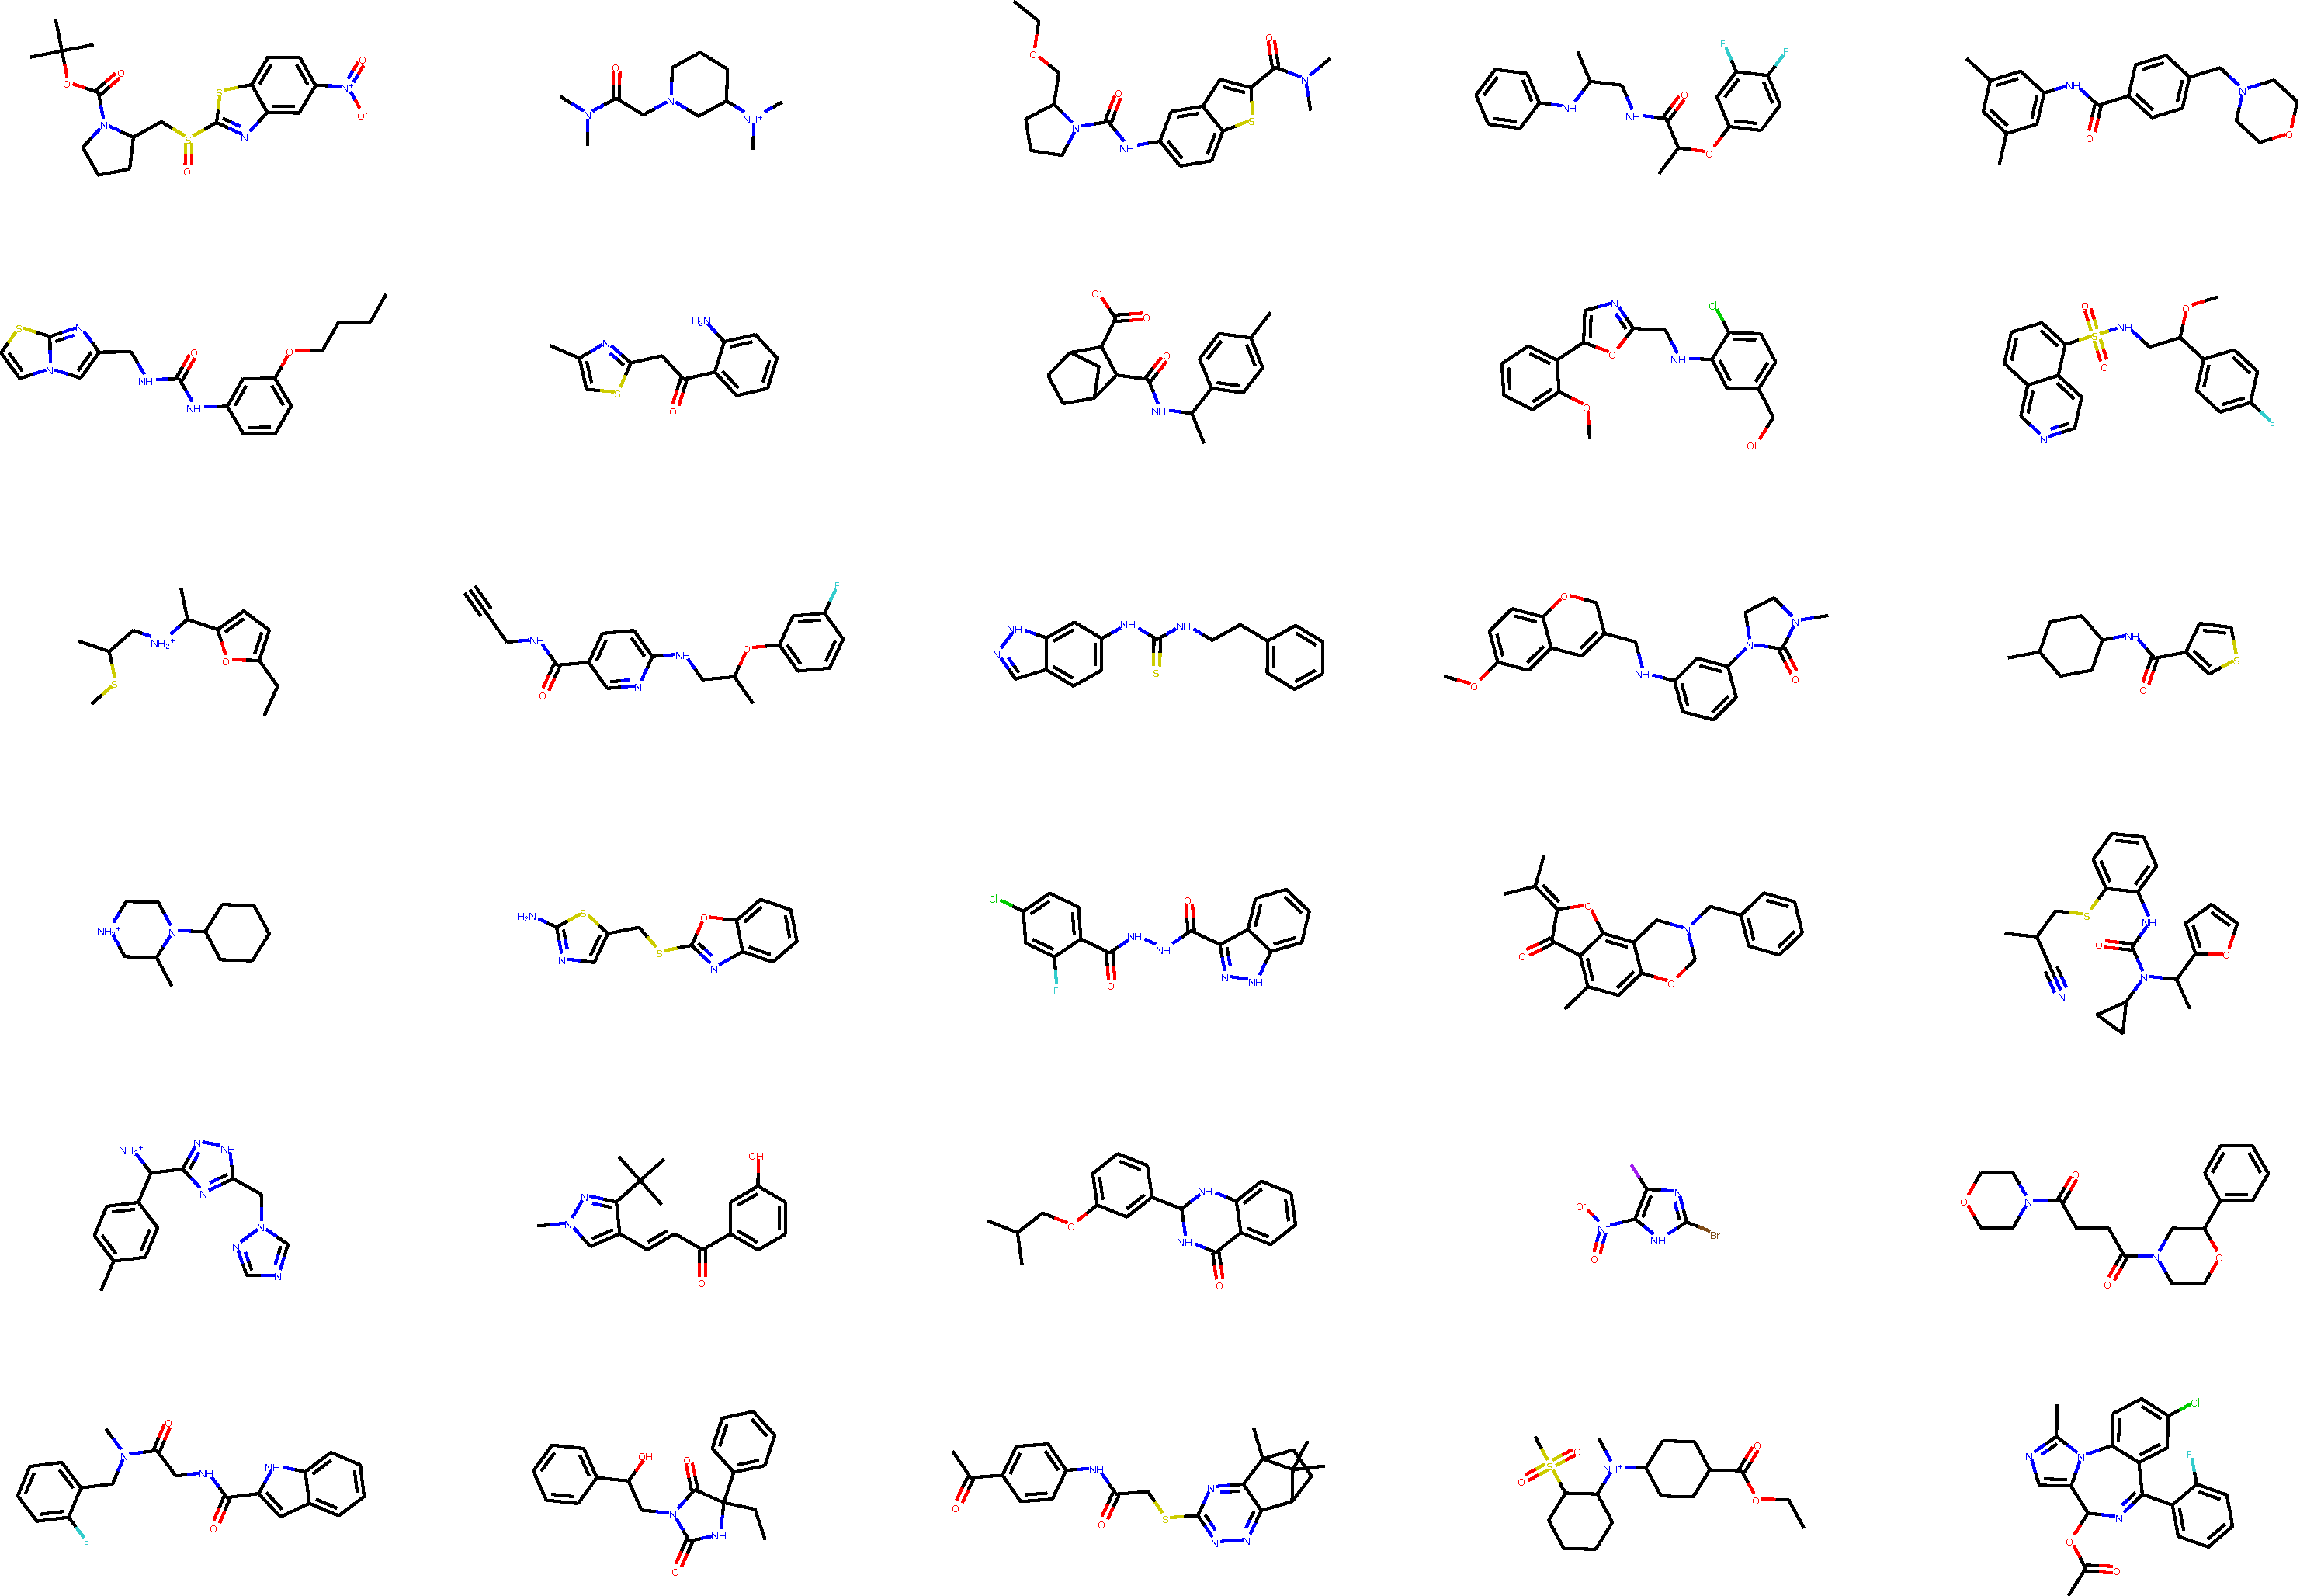
\includegraphics[width=\textwidth]{Figures/Chapter6/samples.eps}
\caption{Five randomly chosen graphs, both from the training sample (left) and generated by our model (right), on each considered dataset (displayed by row). Notice how our generative model has picked up all the characterizing connectivity patterns.}
\label{fig:samples}
\end{figure}

\subsubsection*{Effect of Node Ordering}
As explained before, our first experiment to assess the effect of the different node ordering is to verify if the dataset can be overfit using different ordering strategies. In Figure \ref{fig:loss}, we plot the loss obtained by every variant in the COMMUNITY, EGO and PROTEINS dataset. The figure shows that the models trained with our strategy, the variant of our strategy based on DFS, and the SMILES ordering are able to reach a lower loss than the alternative strategies, which in contrast plateau at higher loss values. This provides evidence that the chosen node ordering strategy is well coupled with the architecture of for our model, and it is sufficiently general to learn connectivity patterns from very different graph datasets. Note that the results of the SMILES ordering are similar to ours as expected. In fact, our node ordering procedure is similar to the way SMILES orders the atoms in a molecular graph. However, we also remark that the SMILES ordering cannot be applied in general, but it is only suitable for molecular graphs.

\begin{figure}[h!]
\centering
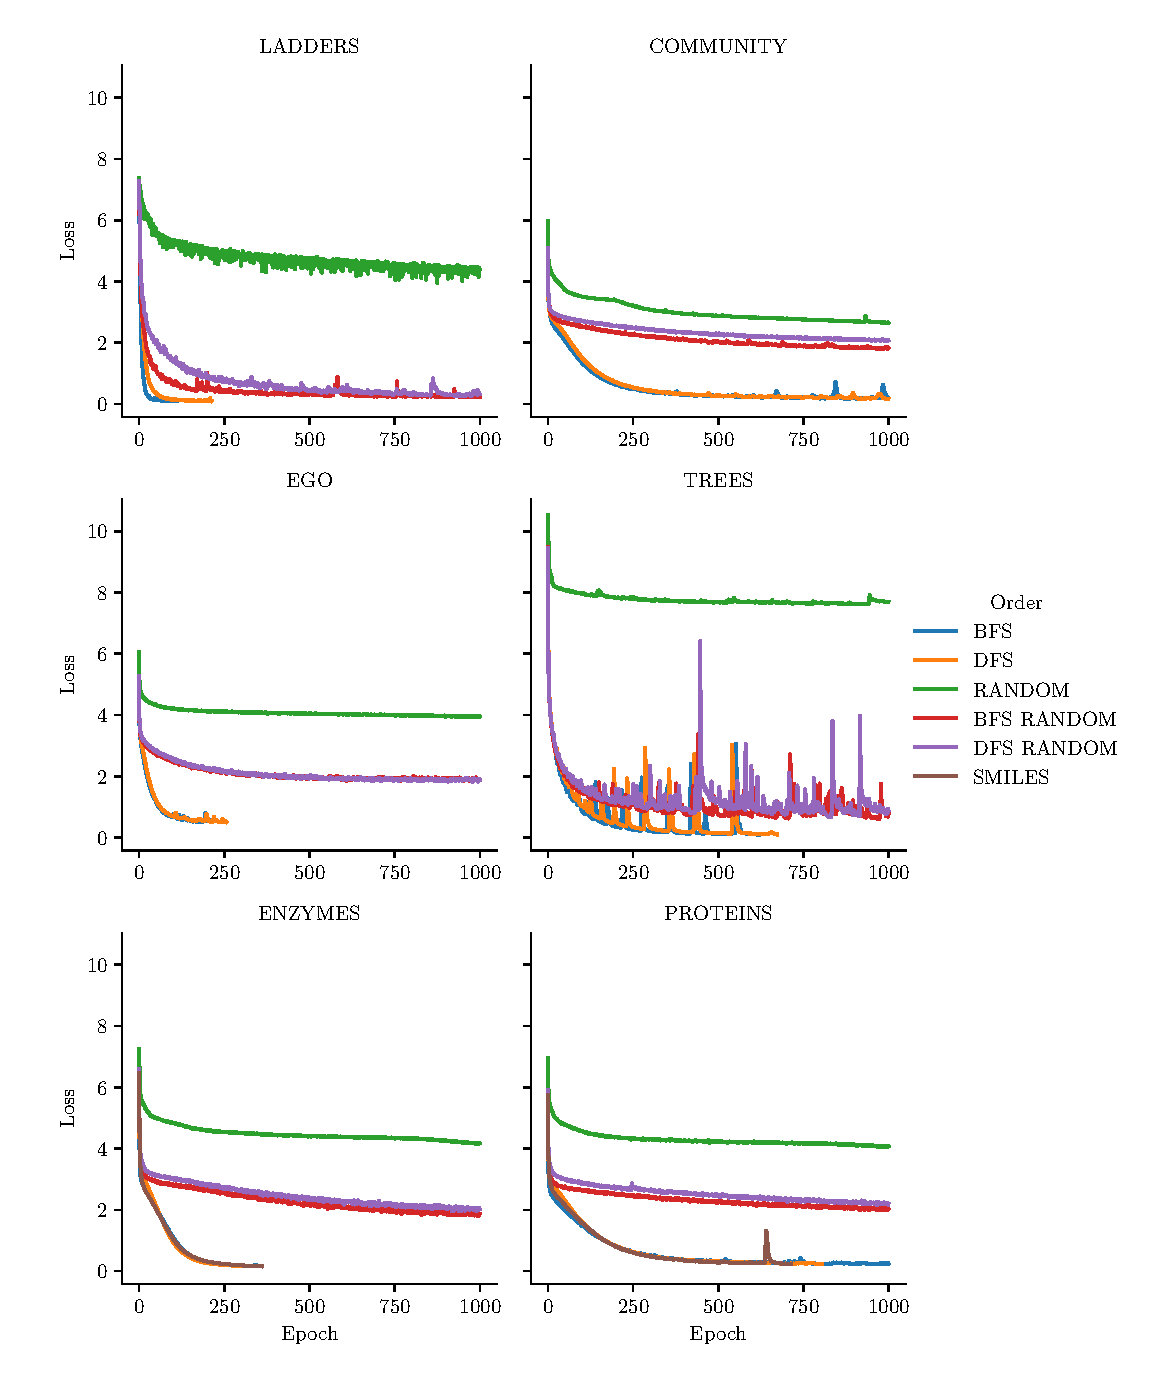
\includegraphics[width=\textwidth]{Figures/Chapter6/loss.eps}
\caption{Plot of the loss on dataset Protein of variants of our approach trained under different node orderings. Notice how the models trained with our proposed node ordering (blue), and SMILES (orange) are able to reach a lower training loss in a smaller number of epochs, compared to variants trained with random ordering (red) and BF random ordering (green).}
\label{fig:loss}
\end{figure}
We complement the discussion about node ordering with a qualitative analysis, whose results are detailed in Table \ref{tab:graph-ordering-qualitative}. It can be easily noticed that the our node ordering strategy yields superior results in every chosen metric, with respect to every other variant. The only competitive node ordering strategy is DF, which basically differs from ours in the way graph nodes are visited. However, despite being able to this strategy seems to underperform in some cases, for example the clustering coefficient in the COMMUNITY dataset and the orbit count in the EGO dataset. We hypothesize this is due to using DF traversal instead of BF, which is less suited to capture local dependencies. In conclusion, these results further extend the evidences supporting the robustness of our approach.
\begin{landscape}
\begin{table}
    \centering
    \caption{Results of the effect of node ordering on the performances of our model. The variants considered are random ordering, Breadth-First (BF) random ordering as proposed in \cite{you2018graphrnn}, SMILES ordering (only for molecular datasets), ordering of the proposed approach. Best performances are bolded.}
    \label{tab:graph-ordering-qualitative}
    \renewcommand{\arraystretch}{1.2}
    \begin{tabular}{lccccccc}
        \toprule
         \textbf{Dataset} & \textbf{Metric} & \textbf{Random} & \textbf{BFS Random} & \textbf{DFS Random} & \textbf{DFS} & \textbf{SMILES} & \textbf{Ours (BFS)}\\
         \midrule
          & ADD           & $0.643 \pm 0.094$ & $0.046 \pm 0.008$ & $0.093 \pm 0.012$ & $0.060 \pm 0.006$ & --                           & $\textbf{0.010} \pm 0.004$\\
          LADDERS & ACC   & $0.340 \pm 0.092$ & $0.031 \pm 0.012$ & $0.036 \pm 0.010$ & $\textbf{0.006} \pm 0.006$ & --                           & $\textbf{0.005} \pm 0.005$\\
          & AOC           & $2.487 \pm 0.403$ & $0.701 \pm 0.151$ & $1.125 \pm 0.145$ & $0.851 \pm 0.160$ & --                           & $\textbf{0.301} \pm 0.100$\\
         \midrule
          & ADD           & $0.038 \pm 0.004$ & $0.041 \pm 0.003$ & $0.054 \pm 0.005$ & $0.044 \pm 0.006$ & --                           & $\textbf{0.017} \pm 0.003$\\
          COMMUNITY & ACC & $1.090 \pm 0.103$ & $0.614 \pm 0.130$ & $2.496 \pm 0.403$ & $0.533 \pm 0.050$ & --                           & $\textbf{0.093} \pm 0.020$\\
          & AOC           & $0.403 \pm 0.026$ & $0.102 \pm 0.009$ & $0.186 \pm 0.019$ & $\textbf{0.054} \pm 0.008$ & --                           & $\textbf{0.054} \pm 0.017$\\
          \midrule
          & ADD           & $0.272 \pm 0.009$ & $0.114 \pm 0.009$ & $0.076 \pm 0.008$ & $0.060 \pm 0.013$ & --                           & $\textbf{0.022} \pm 0.005$\\
          EGO & ACC       & $0.506 \pm 0.034$ & $0.283 \pm 0.018$ & $0.219 \pm 0.049$ & $\textbf{0.078} \pm 0.013$ & --                           & $\textbf{0.066} \pm 0.010$\\
          & AOC           & $0.666 \pm 0.030$ & $0.616 \pm 0.035$ & $0.428 \pm 0.022$ & $0.284 \pm 0.022$ & --                           & $\textbf{0.114} \pm 0.010$\\
         \midrule
          & ADD           & $0.118 \pm 0.009$ & $0.103 \pm 0.007$ & $0.129 \pm 0.006$ & $0.028 \pm 0.003$ & $0.048 \pm 0.008$          & $\textbf{0.017} \pm 0.004$\\
          ENZYMES & ACC   & $1.067 \pm 0.275$ & $0.441 \pm 0.043$ & $0.968 \pm 0.083$ & $\textbf{0.064} \pm 0.014$ & $0.122 \pm 0.022$          & $\textbf{0.054} \pm 0.028$\\
          & AOC           & $0.550 \pm 0.053$ & $0.210 \pm 0.016$ & $0.438 \pm 0.026$ & $\textbf{0.083} \pm 0.018$ & $\textbf{0.134} \pm 0.021$ & $\textbf{0.106} \pm 0.021$\\
         \midrule
          & ADD           & $0.219 \pm 0.009$ & $0.176 \pm 0.007$ & $0.184 \pm 0.006$ & $0.010 \pm 0.011$ & $0.143 \pm 0.009$          & $\textbf{0.059} \pm 0.008$\\
          PROTEINS & ACC  & $0.817 \pm 0.058$ & $0.670 \pm 0.042$ & $0.925 \pm 0.056$ & $0.171 \pm 0.020$ & $0.402 \pm 0.040$          & $\textbf{0.064} \pm 0.017$\\
          & AOC           & $0.594 \pm 0.045$ & $0.202 \pm 0.014$ & $0.319 \pm 0.015$ & $0.069 \pm 0.010$ & $0.217 \pm 0.027$          & $\textbf{0.048} \pm 0.008$\\
         \bottomrule
    \end{tabular}
\end{table}
\end{landscape}


\subsection{Conclusions}
In this work, we have presented a novel generative model for graphs based on Recurrent Neural Networks, which is capable of generating high quality graphs from very different graph distributions. The key idea at the root of our work is to move from the domain of graphs to the one of sequences to simplify the learning task, while retaining most of the expressiveness. Our motivation to frame the generative process as learning problem on sequences is three-fold: (i) it is intuitive, (ii) it allows to work indirectly on smaller and informative portions of the exponentially large graph space, and (iii) it enables the use of the reliable and heavily optimized machinery of Recurrent Neural Networks to learn effectively.

With these ideas in mind, we developed a model which, first, orders nodes in a graph sequentially, then converts graphs into ordered sequences of edges, and finally learns these sequences using two RNNs. The first one predicts a sequence of source nodes, while the second uses the output of the first to predict all necessary endpoints to construct a novel graph. We tested our model against canonical random models from graph theory, a RNN baseline with limited expressiveness, and a state-of-the-art model on five different datasets. The evaluation was conducted on multiple levels, considering both quantitative performance measures such as novelty and uniqueness of generated graphs, as well as qualitative metrics to assess whether generated samples retain structural features of those in the training set. The results clearly show that our model performs at, and sometimes surpasses, the state of the art in the task.
We also conducted a study of how much the procedure chosen to superimpose an order on graph nodes is effective for the particular task of graph generation. More in detail, we compared with 5 variants of our model that were trained on different node orderings. Results show that with the ordering procedure of choice, the model can reach a lower training error, which is essential to learn the complex patterns needed to generate good quality graphs that resemble real-world ones.

The proposed model has also limitations. Even if it works empirically, the constraint imposed by the reliance on a specific ordering is unsatisfactory from a theoretical point of view. For this reason, one key step in future research is to study the node ordering problem more thoroughly, in order to relax and perhaps remove completely such constraint. Another limitation of our approach in its current form is the fact that it is not formulated to include node and edge labels, which are usually found in large classes of graph datasets such as molecular ones. While on one hand this limits the applicability of our approach on those domains, on the other we are also confident that extending the model to include node and edge labels might lead to improvements in generative tasks that deal with those kinds of graphs. Our belief is supported by the intuition that the ability of our model to well approximate structural features of graph distributions, coupled with a reliable mechanism to generate labels, could in perspective improve generalization, since conditioning the generative process not only on structure, but also on features, could help the model learn general connectivity patterns more reliably. This would also allow to compare our model to current molecular graph generator, and investigate the influence of domain specificity on this task.

As for other research directions, we mention the possibility to extend the model by adopting attention mechanisms \citep{bahdanau2015attention}, instead of conditioning the second network only on the last hidden state of the first. Another easily implementable extension of our approach is to model the generative process using a Variational Auto-Encoder in between the two recurrent neural networks, in order to constrain the latent space where the encoding of the first sequence is mapped to be normally distributed. This would have the advantage of cutting sampling time by approximately half, since the inference phase would only require to sample a point from latent space, and decode it using the second network. Lastly, a challenge for the near future is to test whether our approach is capable to scale to larger graphs, which would strengthen our positive results further, as well as expand its applicability to a broader class of problems.
